\documentclass[AER, draftmode]{AEA}

\usepackage{graphicx,float,amssymb, amsmath,titlesec,subcaption,natbib, adjustbox}

\draftSpacing{1.5}
\newtheorem{theorem}{Theorem}[section]
\newtheorem{lemma}[theorem]{Lemma}
\newtheorem{proposition}[theorem]{Proposition}
\newtheorem{corollary}[theorem]{Corollary}

\begin{document}

\title{Economic Growth, Unemployment and Mortality}
\shortTitle{Modelling Mortality with Economic Indicators}
\author{Julien Neves\thanks{Julien Neves: McGill University, 26046227, neves.julien@gmail.com.}}
\date{\today}
\issueName{ECON 647 - Applied Computational Economics}
\pubMonth{April}
\pubYear{2017}
\JEL{J11, C32, E32, I12}
\Keywords{Lee-Carter model; Poisson log-bilinear regression; Gross Domestic Product; Unemployment rate}

\begin{abstract}
Following \cite{Niu2014} and \cite{Brouhns2002} approach, this paper propose an extension of the popular \cite{Lee1992} model for mortality rates to allow for the inclusion of socio-economic variables. Using Canadian data from 1970 to 2009 for mortality, GDP and unemployment, we test different specifications of our model and compare their fit both in-sample and out-of-sample.
\end{abstract}

\maketitle

\section{Introduction}\label{sec:intro}


Life expectancy and mortality rates are essential to understand the world's demographic evolution and aging population. Over the past decades, mortality rates have been declining consistently across the world, which had tremendous repercussion on our current society. Indeed, while a baby born in 1900 would on average die before the age a 50, today the same baby could well live past the age of 80. \cite{Pitacco2009} describe in more details these changes in life expectancy over the years.

The transformations induced by this constant reduction in mortality rates over time have important implications for the design of optimal fiscal and public policies. For example, if the population lives longer, governments must take this into account when planning social benefits and how to fund them for future generations. And while demographic issues are certainly crucial for governments across the world, the private sector is not completely apathetic to this problem. For instance, most life insurances providers' and pension funds' actuarial models rest upon some sort of measure for survival probabilities. And as life expectancy change, so does the cost of longevity risk. Accurate prediction of life expectancy should therefore be a priority in the economic research agenda. 

While the models for mortality rates are plentiful, \citet{Booth2008} classified them into three basic categories: expectative, explanative, and extrapolative. In their simplest form, expectation models are based on experts opinions and their expectation of the future, explanation models are trying to uncover some links between mortality rates and different risk factors, and extrapolative model are based on past trends to infer future outcomes. For an extensive review of available methods for predicting life expectancy, see \citet{Booth2008}.

The most prevalent type of models in the literature are extrapolative models. In particular, \cite{Lee1992} developed the now recognized benchmark model in the field. The method is based on the interrelated mortality dynamics of age and time. Simply put, \cite{Lee1992} model proposed a log-bilinear form for the death rate, which includes both a time and age component. The model is then estimated to match historical data closely. One popular extension of the \cite{Lee1992} model, based on \cite{Alho2000} recommendation, is the Poisson log-bilinear regression approach by \citet{Brouhns2002}. At their core, both methods are similar as the latter is simply the former embedded in Poisson regression approach. 

While other extensions of the \cite{Lee1992} model exist, the \cite{Lee1992} model and the \citet{Brouhns2002} extension are still the most widely used tools for mortality projections. And like the other extrapolative models, they simply aim at extracting a latent factor which can capture historical trend in mortality data. Hence, if past trends cease to continue in the future, these models will not be able to properly quantify possible change in mortality rates. One avenue to circumvent this shortcoming is to confront these latent factors to some observables socio-economic variables, and by doing so, try to bridge the gap between extrapolative and expectative models. Unfortunately, few have attempted this approach, for more details, see \cite{Hanewald2009} and \cite{Niu2014}.

The straightforward method for including socio-economic variables in the \cite{Lee1992} model is to model the time-varying latent factor as an autoregressive process with exogenous socio-economic variables instead of using the usual ARIMA$(p,d,q)$ process. \cite{Hanewald2009} precisely take this approach by including gross domestic product (GDP) variations in an autoregressive modeling of the latent factor. While this method is readily applicable to most extrapolative models, it is only relevant ex-post estimation of the original model. Another approach is that of \cite{Niu2014}, where instead of relating macroeconomics fluctuations to the estimated latent factor of the \cite{Lee1992} model, socio-economics variables are directly included in the \cite{Lee1992} model. Indeed, \cite{Niu2014} encompassed GDP in the log bilinear form of \cite{Lee1992} model.

Note that both \cite{Hanewald2009} and \cite{Niu2014} solely looked at GDP as the driver of mortality rates. Indeed, GDP comes as an easy choice, since there has been a lot of research to study the link between mortality rates and GDP. It is straightforward to see that both variables are linked, and the causality could go in both direction. For some research on this topic, see \cite{Pritchett1996}, \cite{Ettner1996}, \cite{Brenner2005}, \cite{Birchenall2007}, \cite{Swift2011}, \cite{Nandi2012}. In any case, both \cite{Hanewald2009} and \cite{Niu2014} found strong correlation between GDP and mortality rates, which leads us to be incline continue the tradition of including it in our own extension of the \cite{Lee1992} model. Another possibly interesting socio-economic indicator for modeling mortality rates is the unemployment rate. Studies have found causal links between death and unemployment, see \cite{Lundin2010}, \cite{Costa1987}, and \cite{Nylen2001}. 

In this paper, we take \cite{Niu2014} method and extend it to both the \citet{Brouhns2002} Poisson log-bilinear approach instead the \cite{Lee1992} model and by including a more general set of socio-economic variables. While the approach presented is quite general and could possibly be include every variables that driving the mortality rate, the identification of the relevant variables would infeasible in our context. Thus, we will look at a restricted set covariates including both GDP and unemployment rate or only GDP. 

The structure of the remainder of the paper is as follows. In Section \ref{sec:model}, we introduce the relevant mathematical procedures behind \cite{Lee1992} model, \citet{Brouhns2002} extension, \cite{Niu2014} model of mortality rates with economic growth, and our own extension of \citet{Brouhns2002} with covariates. In Section \ref{sec:results}, we apply our model to Canadian mortality and macroeconomics data from 1970 to 2009. Finally, we present a final discussion on the implication of our results in Section \ref{sec:conclusion}.


\section{Model}\label{sec:model}

\subsection{\cite{Lee1992} model} \label{lee}

\cite{Lee1992} famously proposed to model the logarithm of the force of mortality ($\mu_{xt}$), at age $x$ during year $t$, as a linear function of an age effect constant ($\alpha_x$) and the interaction of a time ($\kappa_t$) and age-time ($\beta_x$) parameter:
\begin{align}\label{eq:lee-carter}
\ln(\mu_{xt})=\alpha_x+\beta_x\kappa_t+\epsilon_{xt}.
\end{align} 
where $\epsilon_{xt} \sim I.I.D.(0,\sigma_\epsilon^2)$. Usually, the following constraints are imposed on the parameters $\kappa_t$ and $\beta_x$
\begin{align}
& \sum_t \kappa_t = 0 \\
& \sum_x \beta_t = 1
\end{align}
in order to ensure identification.

This model is usually fitted using an OLS estimation procedure via a single value decomposition method. \cite{Alho2000} suggests that this estimation strategy implies methodological drawbacks, mainly on the basis of the assumption of homoskedasticity, which is too strong because the force of mortality is consistently more variable at older ages. In fact, this is due to inference is being based on assuming normality of the error. One solution to this problem is presented in Section \ref{poisson}.

Note that mortality forecast are based on taking the estimated parameters $\alpha_x$, $\beta_x$ and projecting the latent variable $\kappa_t$.  The latent variable is commonly modeled as an ARIMA$(p,d,q)$ process. \cite{Lee1992}, \cite{Lee2001}, \cite{Hanewald2009}, and others have found that $\kappa_t$ is usually fairly well described by the following unit root process, i.e. $(p,d,q) = (0,1,0)$.
\begin{align}
\kappa_t = \delta + \kappa_{t-1} +u_t
\end{align}
where $\delta$ is a drift term, and $u_t$ a white noise error.

\subsection{Poisson log-bilinear model \citep{Brouhns2002}} \label{poisson}

To circumvent some of the estimation difficulties of the simple \cite{Lee1992} model addressed in Section \ref{lee}, \cite{Brillinger1986} and \cite{Macdonald1996} have shown that a Poisson distribution was well suited to characterize the data generating process of the \cite{Lee1992} model errors. In turn, they proposed that specifying the number of death as a counting random variable could be appropriate, and as such, would simultaneously refined the information set provided to the model. The Poisson extension of the \cite{Lee1992} model, define as a generalized linear model, was successfully applied by \cite{Brouhns2002}, \cite{Hanewald2009} and \cite{Sithole2000}. 

Building on this, one of the most popular extension of the standard extrapolative statistical model of \cite{Lee1992} is the Poisson log-bilinear approach of \cite{Brouhns2002}. The notation here stays close to \cite{Brouhns2002} for consistency purposes.

The model specify
\begin{align}
&D_{xt}\sim\text{Poisson}(E_{xt}\mu_{xt})
\end{align}
where $D_{xt}$ is the observed number of deaths, $\mu_{xt}=exp(\alpha_x+\beta_x\kappa_t)$, is the force of mortality, both recorded at age $x$ during year $t$, while $E_{xt}$ is the exposure-to-risk, i.e., the population distribution. 

The parameters defining $\mu_{xt}$ can be interpreted in the same way as the \cite{Lee1992} model: $\alpha_x$ is the average of the log force of mortality over time; $\beta_x$ indicates the age specific-effect for a given change in the time trend of the log force of mortality; $\kappa_t$ is the time trend of the log force of mortality. The model is estimated by maximum likelihood, based on the following log-likelihood function:
\begin{align}
L(\alpha,\beta,\kappa)=\sum_{x,t}\{D_{xt}(\alpha_x+\beta_x\kappa_t)-E_{xt}exp(\alpha_x+\beta_x\kappa_t)\}+const.
\end{align}
In practice, we let $D_{xt}$ be the observed number of deaths and $\hat{D}_{xt}$ be defined in the following way $\hat{D}_{xt}=E_{xt}exp(\hat{\alpha}_x+\hat{\beta}_x\hat{\kappa}_t)$. 

Standard maximum likelihood Poisson regression methods cannot deal with the bilinear parameter term $\beta_x\kappa_t$. \cite{Goodman1979} proposed a to use a Newton optimization type algorithm to solve the likelihood equation with the following updating scheme
\begin{align}
	\hat{\theta}^{(v+1)}=\hat{\theta}^{(v)}  - \frac{\frac{\partial L^{(v)}}{\partial \theta}}
	{\frac{\partial^2 L^{(v)}}{\partial \theta}}
\end{align}
where $L^{(v)} = L^{(v)}(\hat{\theta}^{(v)})$

In our context, the parameters are solved independently and iteratively using the following procedure from iteration state $v$:
\begin{align}
&\hat{\alpha}_x^{(v+1)}=\hat{\alpha}_x^{(v)}-\frac{\sum_t (D_{xt}-\hat{D}_{xt}^{(v)})}{-\sum_t\hat{D}_{xt}^{(v)}},\;\hat{\beta}_x^{(v+1)}=\hat{\beta}_x^{(v)},\;\hat{\kappa}_t^{(v+1)}=\hat{\kappa}_t^{(v)},\\
&\tilde{\kappa}_t^{(v+2)}=\hat{\kappa}_t^{(v+1)}-\frac{\sum_x(D_{xt}-\hat{D}_{xt}^{(v+1)})\hat{\beta}_x^{(v+1)}}{-\sum_x\hat{D}_{xt}^{(v+1)}(\hat{\beta}_x^{(v+1)})^2},\;\hat{\alpha}_x^{(v+2)}=\hat{\alpha}_x^{(v+1)},\;\hat{\beta}_x^{(v+2)}=\hat{\beta}_x^{(v+1)},\\
&\hat{\kappa}_t^{(v+2)}=\tilde{\kappa}_t^{(v+2)}-(\frac{1}{T}\sum_{s=1}^{T}\tilde{\kappa}_s^{(v+2)}),\\
&\hat{\beta}_x^{(v+3)}=\hat{\beta}_x^{(v+2)}-\frac{\sum_t (D_{xt}-\hat{D}_{xt}^{(v+2)})\hat{\kappa}_t^{(v+2)}}{-\sum_t\hat{D}_{xt}^{(v+2)}(\hat{\kappa}_t^{(v+2)})^2},\;\hat{\alpha}_x^{(v+3)}=\hat{\alpha}_x^{(v+2)},\;\hat{\kappa}_t^{(v+3)}=\hat{\kappa}_t^{(v+2)},
\end{align}
where we can initialize at the parameters in the following way: $\hat{\alpha}_x^{(0)}=0,\;\hat{\beta}_x^{(0)}=1$ and $\hat{\kappa}_t^{(0)}=1$. Random numbers could also be used for the initialization. We stop the iteration process when $L^{(v+1)}(\hat{\alpha}_x^{(v+1)},\hat{\beta}_x^{(v+1)},\hat{\kappa}_t^{(v+1)})-L^{(v)}(\hat{\alpha}_x^{(v)},\hat{\beta}_x^{(v)},\hat{\kappa}_t^{(v)})\leq 10^{-10}$. Again in order for the parameter to be identify, we need to impose the following constraint $\sum_t\kappa_t=0$ and $\sum_x\hat{\beta}_x=1$. The former is ensured by centering the updated $\kappa_t$ parameter estimate as an intermediary step. The latter can be imposed with the normalizations $\bar{\hat{\beta}}_x^{(*)}=\frac{\hat{\beta}_x^{(*)}}{\sum_x\hat{\beta}_x^{(*)}} $ and $\bar{\hat{\kappa}}_t^{(*)}=\hat{\kappa}_t^{(*)}\cdot (\sum_x\hat{\beta}_x^{(*)})$ after the final iterative step (*) with respect to the stopping criteria. The fitted model is defined as:
\begin{align}
\hat{\mu}_{xt}^{(*)}=exp(\hat{\alpha}_x^{(*)}+\bar{\hat{\beta}}_x^{(*)}\bar{\hat{k}}_t^{(*)}).
\end{align}

Naturally the mortality rate can be forecast in the same way as the \cite{Lee1992} model, by using the estimated parameters $\alpha_x$, $\beta_x$ and modeling the latent variable $\kappa_t$ as an ARIMA$(p,d,q)$ process.


\subsection{\cite{Lee1992} model with GDP \citep{Niu2014}}

While modeling $\kappa_t$ as an ARIMA$(p,d,q)$ process does capture some historical trends, as described in Section \ref{sec:intro}, there is some limitations. For example, if the historical trends die out, the ARIMA$(p,d,q)$ process does little to help us forecast the mortality rates in this situation. Hence, we turn our attention to \cite{Niu2014} extension of \cite{Lee1992} model which include an observable time-varying socio-economic variable. The approach described in \cite{Niu2014} is to include a proxy of economic growth in the \cite{Lee1992} model by modifying the log-bilinear model for $\ln(\mu_{xt})$ with the following formula
\begin{align}
\ln(\mu_{xt})=\alpha_x+\beta_x \kappa_t + \gamma_x g_t + \epsilon_{xt}
\end{align} 
where $g_t$ is the real gross domestic product at time $t$, and $\epsilon_{xt}$, $\alpha_x$, $\beta_x$, and $\kappa_t$ have the same interpretation as before if $g_t$ is centered about its mean, i.e. $\frac{1}{T}\sum_{t=1}^T g_t = 0$.

As for the \cite{Lee1992} model, some constraints are needed to identify the parameters. The usual $\sum_t \kappa_t = 0$ and $\sum_x \beta_t = 1$ conditions are sadly not sufficient to identify $\theta = (\alpha_1, ..., \alpha_X, \beta_1, ..., \beta_X, \kappa_1, ..., \kappa_t, \gamma_1,..., \gamma_X)$. In fact, as \cite{Niu2014} showed, we can re-parametrize  $\ln(\mu_{xt})$ for some $c$, $e$, and $d\neq 0$ in the following way
\begin{align}\label{eq:par_1}
\begin{split}
	\ln(\mu_{xt}) &= \alpha_x+\beta_x \kappa_t + \gamma_x g_t \\
	&= \alpha_x+\beta_x (\kappa_t - eg_t)+ (\gamma_x + e\beta_x) g_t \\
	&= (\alpha_x-\beta_xc)+\frac{\beta_x}{d} (d(\kappa_t - eg_t+c))+ (\gamma_x + e\beta_x) g_t \\
	&= \tilde{\alpha}_x+\tilde{\beta}_x \tilde{\kappa}_t + \tilde{\gamma}_x g_t
\end{split}
\end{align}
where
\begin{align}
\tilde{\alpha}_x &= \alpha_x - \beta_x c\\
\tilde{\beta}_x &= \frac{\beta_x}{d} \\
\tilde{\kappa}_t &= d(\kappa_t - eg_t+c)\\
\tilde{\gamma}_x &= \gamma_x + e\beta_x
\end{align}

Therefore, to uniquely identify $\theta = (\alpha_1, ..., \alpha_X, \beta_1, ..., \beta_X, \kappa_1, ..., \kappa_t, \gamma_1,..., \gamma_X)$, \cite{Niu2014} proposed the following constraints
\begin{align} \label{eq:con_1}
& \sum_t \kappa_t = 0 \\ \label{eq:con_2}
& \sum_x \beta_t = 1 \\ \label{eq:con_3}
& cov(\kappa_t, g_t) = 0 \\ \label{eq:con_4}
& \kappa = (\kappa_1,..., \kappa_T) \neq 0
\end{align}

To show that \ref{eq:con_1}, \ref{eq:con_2}, \ref{eq:con_3}, and \ref{eq:con_4} are sufficient to identify $\theta$, \cite{Niu2014}, following \cite{Nielsen2010}, proved the following theorem 
\begin{theorem}\label{the:1}
	Let $m = (\ln(\mu_{xt}), x = 1,..., X, t = 1, ..., T)$, where $m = m(\theta)$ satisfies $\ln(\mu_{xt}) = \alpha_x + \beta_x \kappa_t + \gamma_x g_t$ for some $\theta = (\alpha_1, ..., \alpha_X, \beta_1, ..., \beta_X, \kappa_1, ..., \kappa_t, \\ \gamma_1,..., \gamma_X)$. Then the parametrization $\theta^o$ where $\sum_{x=1}^{X} \beta_x^o = 1$, $\sum_{t=1}^{T} \kappa_t^o = 1$, $cov(\kappa_t^o, g_t)=0$ in sample, and $\kappa^o \neq 0$, satisfies
	\begin{enumerate}
		\item[(i)] $\theta^o$ is a function of $\theta$
		\item[(ii)] $m$ is a function of $\theta$ through $\theta^o$
		\item[(iii)] The parametrization of $m$ by $\theta^o$ is exactly identified. That is, if $\theta^1 \neq \theta_2$ are two parameters satisfying the normalizing constraints, then $m(\theta^1) \neq m(\theta^2)$.
	\end{enumerate}
\end{theorem}

Using Theorem \ref{the:1}, it is straight forward to show that \ref{eq:con_1}, \ref{eq:con_2}, \ref{eq:con_3}, and \ref{eq:con_4} do in fact uniquely identify $\theta$. We reproduced \cite{Niu2014} proof of Theorem \ref{the:1} in the appendix for the convenience of the reader.

Now, to estimate this model, the usual singular value decomposition technique used in \cite{Lee1992} is not feasible. To remedy this problem, \cite{Niu2014} used a modified version of the weighted least squares technique proposed by \cite{Wilmoth1993} for the \cite{Lee1992}. For more details on how to estimate using the weighted least squares technique, see \cite{Wilmoth1993}.

Like the \cite{Lee1992} model and \cite{Brouhns2002} extension, mortality forecast are based on taking the estimated parameters $\alpha_x$, $\beta_x$ and projecting the latent variable $\kappa_t$. Again, the latent variable is commonly modeled as an ARIMA$(p,d,q)$ process. The difference in \cite{Niu2014} approach is that GDP also needs to be forecast. While there is no restrictions on how to forecast $g_t$, a simple approach is to also fit an ARIMA$(p,d,q)$ model to the $g_t$. Note that we can't forecast $g_t$ and $\kappa_t$ jointly using, for example, a VAR$(p)$ model, because by construction $cov(\kappa_t, g_t) = 0$.

\subsection{Poisson log-bilinear model with covariates} \label{model}

In this section, we extend the Poisson log-bilinear approach of \cite{Brouhns2002} to include some covariates such as economic growth as in \cite{Niu2014}. The difference in our approach is that instead of restring ourselves to only $g_t$, we include a set of $k$ covariates namely $Y$ where
\begin{align}
	Y = \begin{bmatrix}
	Y'_1 \\
	... \\
	Y'_t \\
	... \\
	Y'_T
	\end{bmatrix}
\end{align}
where $Y'_t$ is an 1 by $k$ matrix. Then, \cite{Brouhns2002} approach can be extended by letting again
\begin{align}
&D_{xt}\sim\text{Poisson}(E_{xt}\mu_{xt})
\end{align}
where $D_{xt}$ is the observed number of deaths, $E_{xt}$ is the exposure-to-risk, i.e., the population distribution, but the force of mortality is now $\mu_{xt}=exp(\alpha_x+\beta_x \kappa_t + \gamma_x Y_t)$. 
Note that $\gamma_x$ is not a vector anymore, but a $X$ by $k$ matrix.

If $Y$ is such that that the columns means are equal to $0$, then the parameters $\alpha_x$ and $\beta_x$ can be interpreted as before. Thus in the spirit of comparisons, if given a matrix of covariate $\tilde{Y}$, it is useful to re-parametrize in the following way
\begin{align}
Y = \begin{bmatrix}
\tilde{Y}_1' - \frac{\sum_{t=1}^{T} \tilde{Y}'_t}{T} \\
... \\
\tilde{Y}_t' - \frac{\sum_{t=1}^{T} \tilde{Y}'_t}{T} \\
... \\
\tilde{Y}_T' - \frac{\sum_{t=1}^{T} \tilde{Y}'_t}{T}
\end{bmatrix}
\end{align}

Before proceeding to the estimation method, we turn our attention to the problem of identification in this model. In fact, we can rewrite $\mu_{xt}$ for some $c$, $e$ and $d\neq 0 $ in the following way
\begin{align}\label{eq:par_2}
\begin{split}
ln(\mu_{xt}) &= \alpha_x+\beta_x \kappa_t + \gamma_x Y'_t \\
&= \alpha_x+\beta_x (\kappa_t - eY'_t)+ (\gamma_x + e\beta_x)Y'_t \\
&= (\alpha_x-\beta_xc)+\frac{\beta_x}{d} (d(\kappa_t - eY'_t+c))+ (\gamma_x + e\beta_x) Y'_t \\
&= \tilde{\alpha}_x+\tilde{\beta}_x \tilde{\kappa}_t + \tilde{\gamma}_x Y'_t
\end{split}
\end{align}
where
\begin{align}
\tilde{\alpha}_x &= \alpha_x - \beta_x c\\
\tilde{\beta}_x &= \frac{\beta_x}{d} \\
\tilde{\kappa}_t &= d(\kappa_t - eY'_t+c)\\
\tilde{\gamma}_x &= \gamma_x + e\beta_x
\end{align}

Then, to be able to identify uniquely $\alpha_x$, $\beta_x$, $\kappa_t$ and $\gamma_x$, we need the following constraints:
\begin{align}
& \sum_x \beta_t = 1 \\ \label{eq:beta_2}
& \sum_x \beta_t = 1 \\ \label{eq:alpha_2}
& cov(\kappa_t, Y'_t) = 0 \\ \label{eq:cov_2}
& \bar{Y} = [\iota \ Y] \text{ has full column rank} \\ \label{eq:col_2}
& \kappa = (\kappa_1,..., \kappa_T) \neq 0 
\end{align}

Note that \ref{eq:cov_2} is included to ensure that $var(Y'_t)$ is not singular and that no linear combination of some columns of $Y$ is equal to the constant, which would prevent us from identifying $\alpha_x$. The fact that $\alpha_x$, $\beta_x$, $\kappa_t$ and $\gamma_x$ are uniquely identified given these constraints holds from the following theorem:
\begin{theorem}\label{the:2}
	Let $m = (ln(\mu_{xt}), x = 1,..., X, t = 1, ..., T)$, where $m = m(\theta)$ satisfies $ln(\mu_{xt}) = \alpha_x + \beta_x \kappa_t + \gamma_x Y_t$ for some $\theta = (\alpha_1, ..., \alpha_X, \beta_1, ..., \beta_X, \kappa_1, ..., \kappa_t, \\ \gamma_1,..., \gamma_X)$. Then the parametrization $\theta^o$ where $\sum_{x=1}^{X} \beta_x^o = 1$, $\sum_{t=1}^{T} \kappa_t^o = 1$, $cov(\kappa_t^o, Y'_t)=0$ in sample, $[\iota \ Y]$ has full column rank, and $\kappa^o \neq 0$, satisfies
	\begin{enumerate}
		\item[(i)] $\theta^o$ is a function of $\theta$
		\item[(ii)] $m$ is a function of $\theta$ through $\theta^o$
		\item[(iii)] The parametrization of $m$ by $\theta^o$ is exactly identified. That is, if $\theta^1 \neq \theta_2$ are two parameters satisfying the normalizing constraints, then $m(\theta^1) \neq m(\theta^2)$.
	\end{enumerate}
\end{theorem}
The proof is given in the appendix.

Now, the model can be estimated by maximum likelihood, based on the following log-likelihood function
\begin{align}
L(\alpha,\beta,k)=\sum_{x,t}\{D_{xt}(\alpha_x+\beta_xk_t+ \gamma_x Y_t)-E_{xt}exp(\alpha_x+\beta_xk_t+ \gamma_x Y_t)\}+const.
\end{align}
where $D_{xt}$ is the observed number of deaths.

As a matter of fact, to simplify our estimation procedure, it is a good idea to rewrite the $\mu_{xt}$ in the following way
\begin{align}
\mu_{xt}=exp(\beta_x \kappa_t + \delta_x \bar{Y}_t)
\end{align}
where $\bar{Y} = [\iota, \ Y]$ and $\delta =[\alpha, \ \gamma]$.

Then, the log-likelihood function becomes
\begin{align}
L(\alpha,\beta,k)=\sum_{x,t}\{D_{xt}(\beta_x \kappa_t + \delta_x \bar{Y}_t)-E_{xt}exp(\beta_x \kappa_t + \delta_x \bar{Y}_t)\}+const.
\end{align}
Additionally, we let $\hat{D}_{xt}=E_{xt}exp(\hat{\alpha}_x+\hat{\beta}_x\hat{k}_t+ \hat{\gamma}_x Y_t)$. 

Once more, standard maximum likelihood Poisson regression methods cannot deal with the bilinear parameter term $\beta_xk_t$, and we use \cite{Goodman1979} Newton-Rhapson approach to solve the likelihood equation. 
\begin{align}
&\hat{\delta}_x^{(v+1)}=\hat{\delta}_x^{(v)}-\frac{\sum_t (D_{xt}-\hat{D}_{xt}^{(v)})\bar{Y}_t}{-\sum_t\hat{D}_{xt}^{(v)}(\bar{Y}_t\circ \bar{Y}_t)},\; \hat{\beta}_x^{(v+1)}=\hat{\beta}_x^{(v)},\;\hat{\kappa}_t^{(v+1)}=\hat{\kappa}_t^{(v)}\\
&\tilde{\kappa}_t^{(v+2)}=\hat{\kappa}_t^{(v+1)}-\frac{\sum_x(D_{xt}-\hat{D}_{xt}^{(v+1)})\hat{\beta}_x^{(v+1)}}{-\sum_x\hat{D}_{xt}^{(v+1)}(\hat{\beta}_x^{(v+1)})^2},\; \hat{\delta}_x^{(v+2)}=\hat{\delta}_x^{(v+1)},\;\hat{\beta}_x^{(v+2)}=\hat{\beta}_x^{(v+1)},\\
&\hat{\kappa}^{(v+2)}=\tilde{\kappa}^{(v+2)}-\bar{Y}(\bar{Y}'\bar{Y})^{-1}\bar{Y}'\tilde{\kappa}^{(v+2)},\\ \label{eq:proj_2}
&\hat{\beta}_x^{(v+3)}=\hat{\beta}_x^{(v+2)}-\frac{\sum_t (D_{xt}-\hat{D}_{xt}^{(v+2)})\hat{\kappa}_t^{(v+2)}}{-\sum_t\hat{D}_{xt}^{(v+2)}(\hat{kappa}_t^{(v+2)})^2},\; \hat{\delta}_x^{(v+3)}=\hat{\delta}_x^{(v+2)},\;\hat{\kappa}_t^{(v+3)}=\hat{\kappa}_t^{(v+2)},
\end{align}
where $\bar{\kappa} = \begin{bmatrix}
\kappa_1\\
...\\
\kappa_T
\end{bmatrix}$ and $(\bar{Y}_t\circ \bar{Y}_t) = \begin{bmatrix}
1, \ (Y)_{t,1}(Y)_{t,1}, & ..., & (Y)_{t,k}(Y)_{t,k}
\end{bmatrix}$. As before,
we can initialize at the parameters in the following way: $\hat{\alpha}_x^{(0)}=0,\;\hat{\beta}_x^{(0)}=1$ and $\hat{k}_t^{(0)}=1$, but random numbers could also be used for the initialization. We stop the iteration process when $\widehat{L}^{(v+1)}(\hat{\alpha}_x^{(v+1)},\hat{\beta}_x^{(v+1)},\hat{\kappa}_t^{(v+1)},\hat{\gamma}_t^{(v+1)})-\widehat{L}^{(v)}(\hat{\alpha}_x^{(v+1)},\hat{\beta}_x^{(v)},\hat{\kappa}_t^{(v)},\hat{\gamma}_t^{(v)})\leq 10^{-10}$. In order for the parameter to be identify, we first need to impose the following constraints $\frac{1}{T}\sum_t\kappa_t = 0$ and $cov(\kappa_t, Y'_t) = 0 $. This is ensured by projecting the updated $\kappa_t$ parameter estimates with the matrix $M = I-\bar{Y}(\bar{Y}'\bar{Y})^{-1}\bar{Y}'$ as an intermediary step. Moreover, $\sum_x \beta_x = 1$ can be imposed with the normalizations $\bar{\hat{\beta}}_x^{(*)}=\frac{\hat{\beta}_x^{(*)}}{\sum_x\hat{\beta}_x^{(*)}} $ and $\bar{\hat{k}}_t^{(*)}=\hat{k}_t^{(*)}\cdot (\sum_x\hat{\beta}_x^{(*)})$ after the final iterative step (*) with respect to the stopping criteria. The fitted model is defined as:
\begin{align}
\hat{\mu}_{xt}^{(*)}=exp(\bar{\hat{\beta}}_x^{(*)}\bar{\hat{k}}_t^{(*)}+ \hat{\delta}_x^{(*)}\bar{Y}_t).
\end{align}
Note that the constraint that $\bar{Y}$ as full column rank is not really imposed anywhere, but it is needed in order for $(\bar{Y}'\bar{Y})^{-1}$ to be non-singular when projecting $\kappa$ with $I-\bar{Y}(\bar{Y}'\bar{Y})^{-1}\bar{Y}'$.

Like the previous models, mortality forecast are based on taking the estimated parameters $\alpha_x$, $\beta_x$, projecting the latent variable $\kappa_t$ and the covariates. Again $\kappa_t$ is modeled with ARIMA$(p,d,q)$ process. For the covariates, any appropriate technique to forecast them can be considered. One approach is to model the covariates as a VAR$(p)$ process and forecast using the estimated coefficients of that model. Note, as in \cite{Niu2014}, covariates and $\kappa_t$ need to be separately modeled, because by construction $cov(\kappa_t, Y_t') = 0$.


\section{Results} \label{sec:results} 

\subsection{Data}

We used mortality data from the Human Mortality Database. For more information about the Human Mortality Database, see http://www.mortality.org. We used the data series for Canada from 1970 to 2009 and for age 0 to 99 years old. 

For the macroeconomic variables, we used data from the OECD database. Both the gross domestic product and unemployment rate for Canada from 1970 to 2009 are readily available from this database. Note that the OECD provide both the unemployment rates for male and female, which is quite useful when estimating for both sex separately In addition, for estimation purposes, we log-linearized the gross domestic product. For more information about the OECD database, see http://stats.oecd.org


\subsection{Estimation Results}

We estimated the \cite{Brouhns2002} Poisson log-bilinear model and our extension using the Newton-Rhapson approach described in Section \ref{sec:model}. Note that the covariates series are centered about their means in order to keep the interpretation of $\alpha_x$ and $\beta_x$ constant. Moreover, we only used part of the sample, i.e. from 1970 to 1999, to estimate the model.

Inherent differences in both male and female life expectancies lead us to model them separately, as most researcher previously did. Graphical representations of the estimated values for the parameters of the model presented in Section \ref{model} for Canadians males is given here in Figure 1. The same figures for Canadian females estimation is given in the appendix in Figure 4.

\begin{figure}[!htp]
	\begin{subfigure}{0.4\textwidth}
		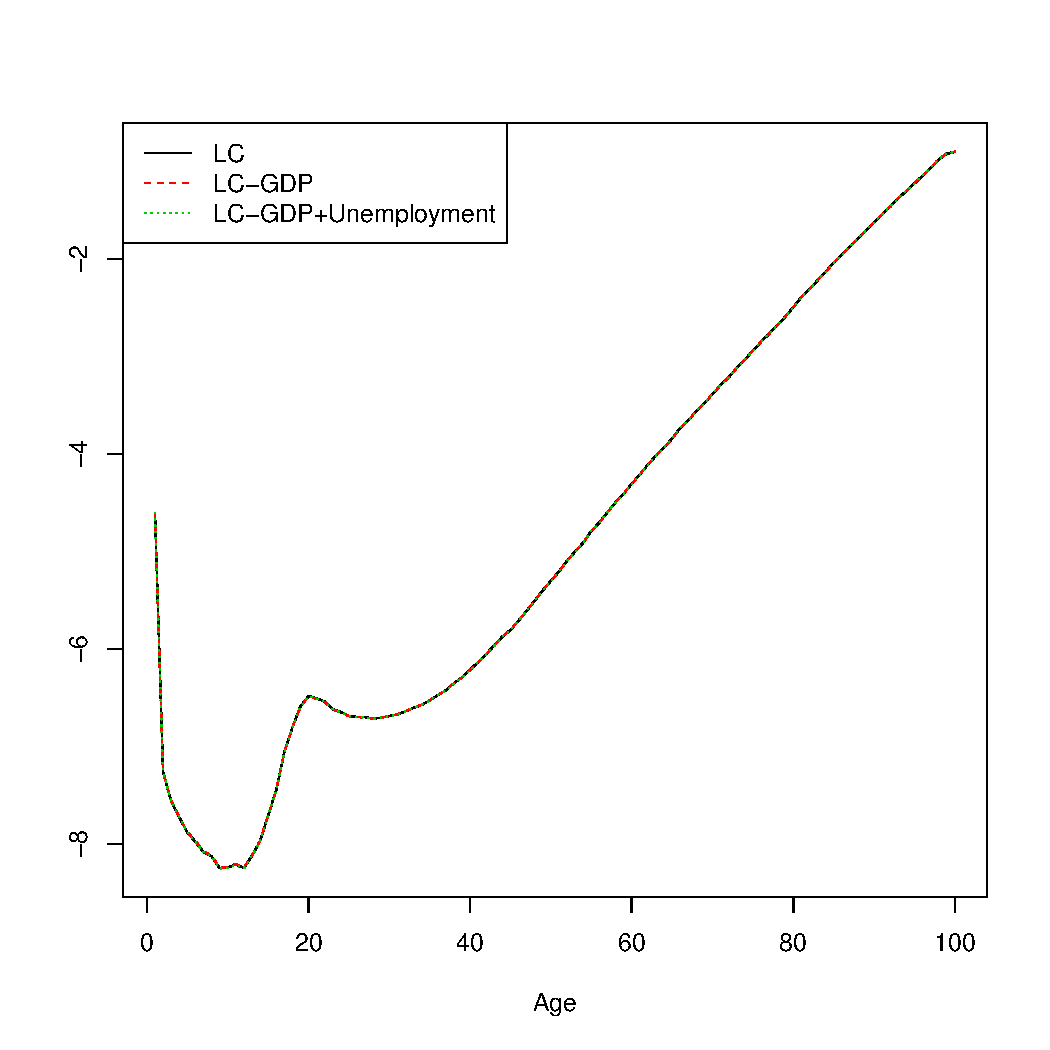
\includegraphics[width=\linewidth]{CAN_ax_male}
		\caption{$\alpha_x$}
		\label{fig:malea}
	\end{subfigure}
	\begin{subfigure}{0.4\textwidth}
		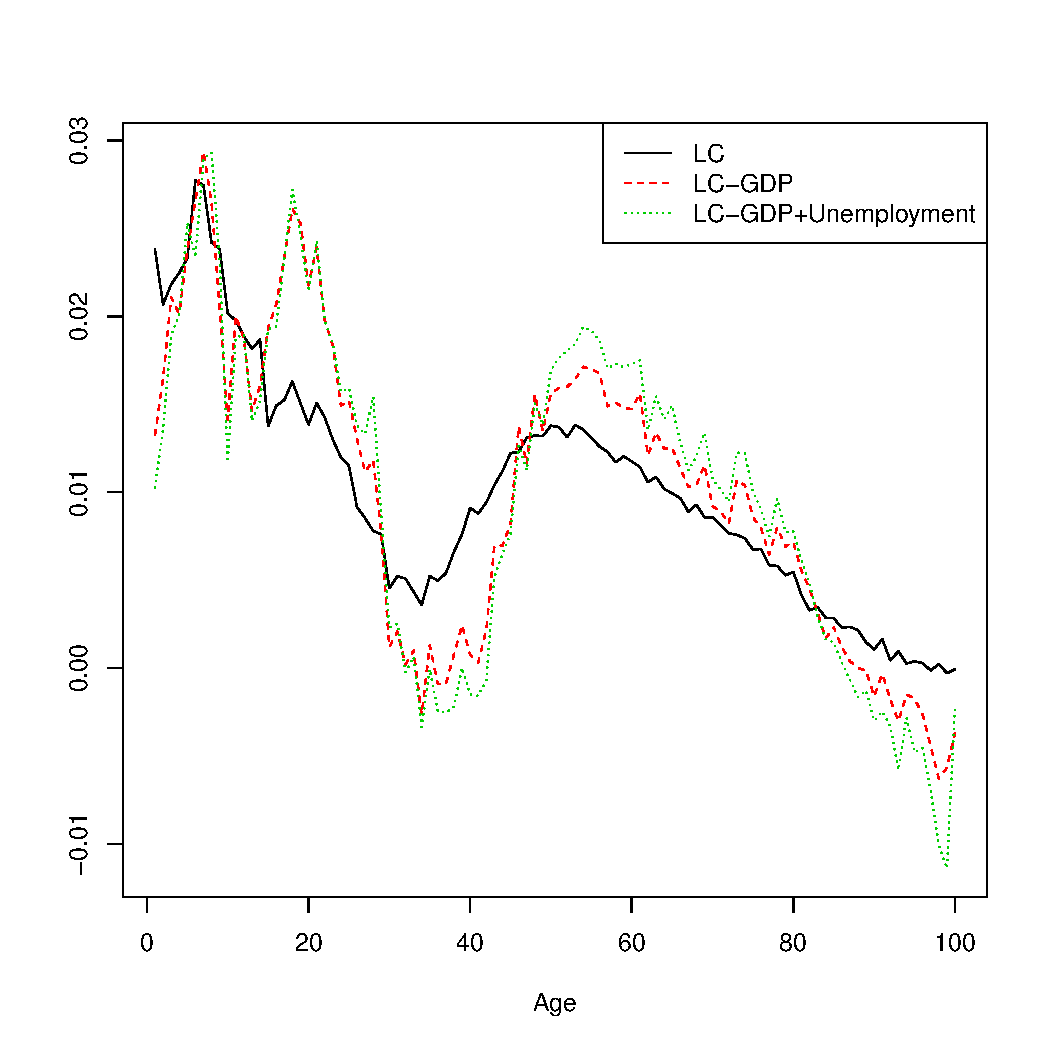
\includegraphics[width=\linewidth]{CAN_bx_male}
		\caption{$\beta_x$}  
		\label{fig:maleb}
	\end{subfigure}
	\begin{subfigure}{0.4\textwidth}
		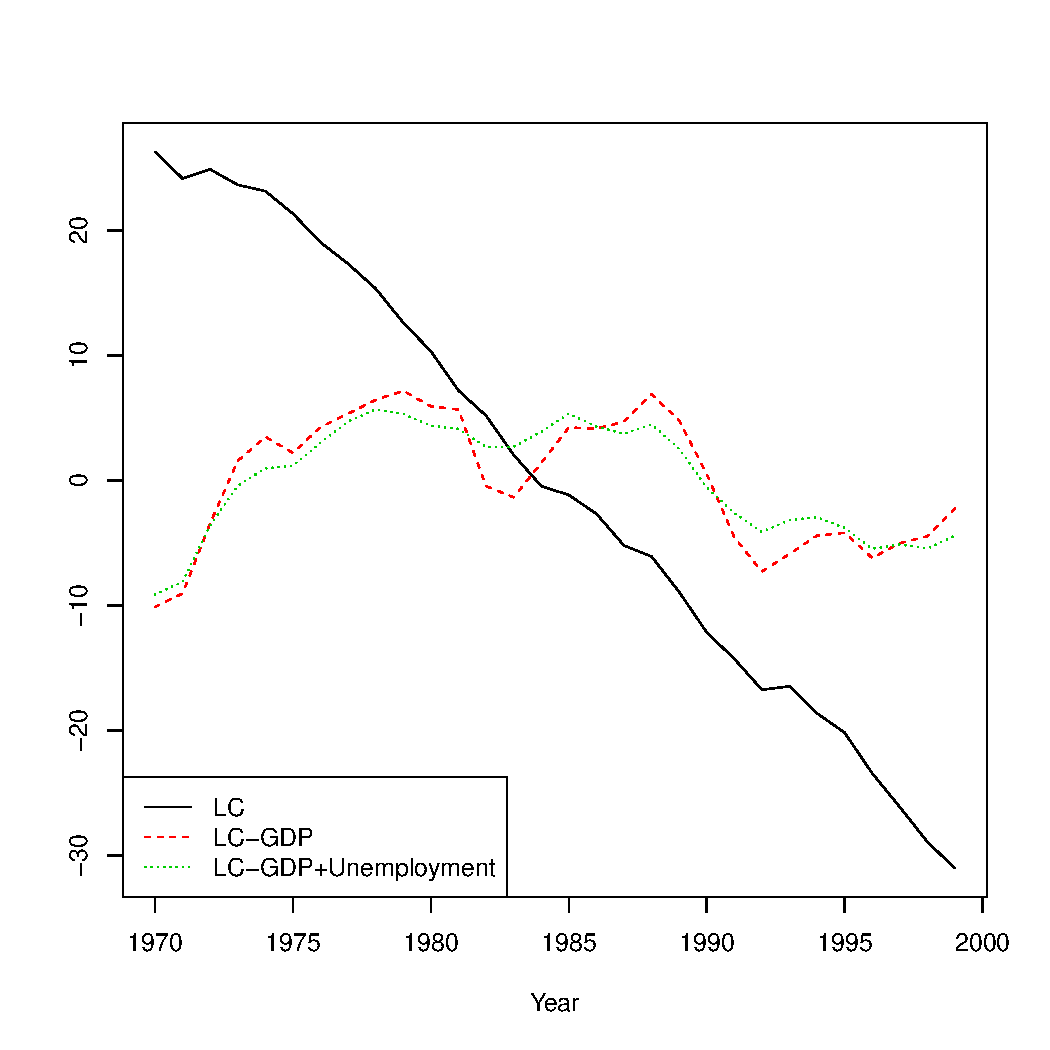
\includegraphics[width=\linewidth]{CAN_kt_male}
		\caption{$\kappa_t$}
		\label{fig:malec} 
	\end{subfigure}
	\begin{subfigure}{0.4\textwidth}
		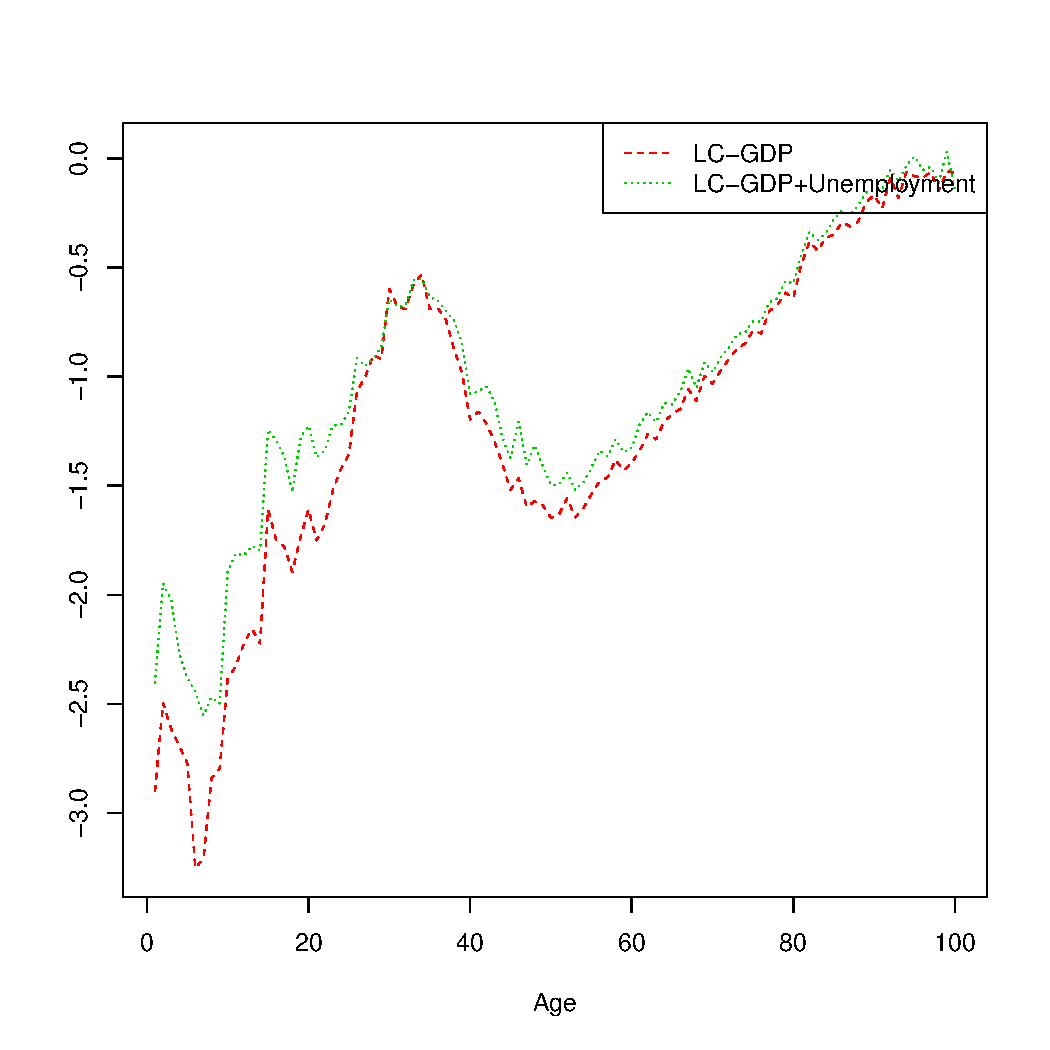
\includegraphics[width=\linewidth]{CAN_g1x_male}
		\caption{$\gamma_{x,gdp}$} 
		\label{fig:maled}
	\end{subfigure}
	\begin{subfigure}{0.4\textwidth}
		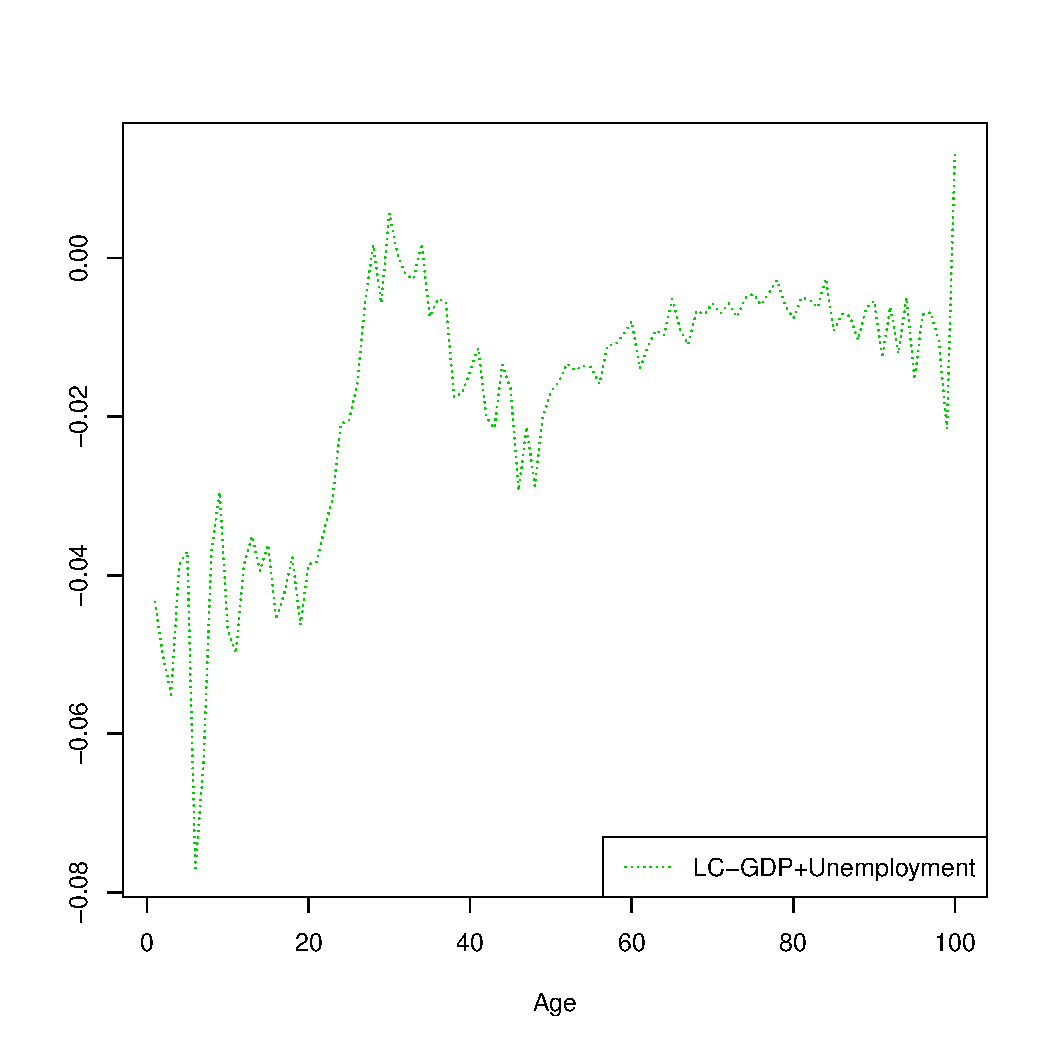
\includegraphics[width=\linewidth]{CAN_g2x_male} 
		\caption{$\gamma_{x,unemployment}$} 
		\label{fig:malee}
	\end{subfigure}
	\caption{Poisson log-bilinear extension with covariates for Canadian males}
\end{figure}

Looking at $\alpha_x$ in Figure \ref{fig:malea} and Figure \ref{fig:femalea} , we can see that all three models give a similar close fit, which we expected as the covariates are centered about their means. In fact, since $\frac{1}{T}\sum_t \kappa_t = 0$ and $\frac{1}{T}\sum_t Y'_t = 0$, we have that  $\alpha_x =\frac{1}{T} \sum_t \ln(\mu_{xt})$.

In turn, the $\beta_x$, i.e. the age-specific patterns of change in $\kappa_t$, goes to 0 as $x$ increases. This indicates that $\ln(\mu_{xt})$ is less sensitive to change in $\kappa_t$ for higher $x$. Note that including covariates increase the volatility of $\beta_x$ as now some of the age-specific patterns are capture by change in the covariates.

The real difference between models comes from the $\kappa_t$. In the original model, $\kappa_t$ captures the decreasing mortality rate over time as seen in Figure \ref{fig:malec} and Figure \ref{fig:femalec}. But, when including covariates, $\kappa_t$ oscillates around 0, indicating that GDP and the combination of GDP and unemployment are able to capture some, if not all, the decreasing mortality rates time trend.

Finally, looking at $\gamma_x$, we see that for both GDP and unemployment an upward trajectory in the estimates reverting to 0 from 0 to 99 years, indicating that the sensitivity of mortality rates on covariates is decreasing over time. We get the same pattern for $\beta_x$, but flipped about the x-axis.


\subsection{In-Sample test}

Two measure of goodness-of-it commonly used by practitioners are the Akaike information criterion (AIC) and the Bayesian information criterion (BIC). The AIC is given by the following formula
\begin{align}
AIC = 2 K - 2 \hat{L}
\end{align}
where $K$ is the number of free parameters and $\hat{L}=\hat{L}(\hat{\alpha}, \hat{\beta}, \hat{\kappa}, \hat{\gamma})$ is the log-likelihood of the estimated model. Note that $K$ is given by $(2+k)X + T - (k+2)$ where $k$ is the number of covariates, $X$ is the number of ages sampled and $T$ is the number of time periods.

On the other hand the BIC is given by this formula
\begin{align}
	BIC = ln(N) K - 2 \hat{L}
\end{align}
where $N$ is the number of observations, $K$ is the number of free parameters and $\hat{L}=\hat{L}(\hat{\alpha}, \hat{\beta}, \hat{\kappa}, \hat{\gamma})$ is the log-likelihood of the estimated model. Note that $K$ has the same value as for the $AIC$ and $N=X\cdot T$. 

Since both measures are based on the log-likelihood; the smaller the measure, the better the model relative to the other models given. The main difference between the AIC and BIC is that the BIC penalize more for the inclusion of more parameters, i.e. higher $K$. Results for the three models are reported in Table \ref{tab:aic}

\begin{table}[!htp]
	\centering
	\caption{AIC and BIC for the Poisson log-bilinear model with covariates}
	\label{tab:aic}
	\begin{tabular}{lllll}
		\hline
		Model                                                              & \multicolumn{2}{l}{Male} & \multicolumn{2}{l}{Female} \\ \cline{2-5} 
		& $AIC$      & $BIC$      & $AIC$       & $BIC$       \\ \hline
		$\alpha_x + \beta_x \kappa_t$                                      & 27420375   & 27421756*   & 22055929    & 22057310*    \\
		$\alpha_x + \beta_x \kappa_t + \gamma_{1x} g_t$                    & 27419816   & 27421798   & 22055958    & 22057940    \\
		$ \alpha_x + \beta_x \kappa_t + \gamma_{1x} g_t + \gamma_{2x} u_t$ & 27419442*   & 27422025   & 22055631*    & 22058214    \\ \hline
	\end{tabular}
\end{table}


Looking at Table \ref{tab:aic}, it seems that AIC and the BIC give opposing view. The AIC seems to prefer models including both covariates, while the BIC indicates that the original model provided a better fit. Therefore, the size of the penalty for the number of parameters induce different model pick for the AIC and BIC.

In addition to the AIC and BIC, we report the likelihood-ratio statistic $(L^2)$ in Table \ref{tab:l2}. The likelihood-ratio statistic is obtained by comparing the current model with an saturated model, and in this context is given by
\begin{align}
	L^2 = 2 \sum_{x} \sum_t D_{xt} \ln \left( \frac{D_{xt}}{\hat{D}_{xt}} \right)
\end{align}
where $\hat{D}_{xt}$ is the estimated number of deaths from the model we are testing. In a sense, this $L^2$ is the opposite of a goodness-of-fit test, i.e. the higher the statistic, the worst the fit.

\begin{table}[!htp]
	\centering
	\caption{$L^2$ for the Poisson log-bilinear model with covariates}
	\label{tab:l2}
	\begin{tabular}{lllll}
	\hline
	Model                                                              & \multicolumn{2}{l}{Male} & \multicolumn{2}{l}{Female} \\ \cline{2-5} 
	& $L^2$    & $\Delta L^2$ & $L^2$       & $\Delta$    \\ \hline
	$\alpha_x + \beta_x \kappa_t$                                      & 5073.87  &              & 4056.46     &             \\
	$\alpha_x + \beta_x \kappa_t + \gamma_{1x} g_t$                    & 4171.78  & 0.178        & 3854.60     & 0.050       \\
	$ \alpha_x + \beta_x \kappa_t + \gamma_{1x} g_t + \gamma_{2x} u_t$ & 3913.91  & 0.229        & 3224.59     & 0.205       \\ \hline
	\end{tabular}
\end{table}

We can see from Table \ref{tab:L2} that including more covariates, does indeed reduce the $L^2$ test. For comparison purposes, we also include $\Delta L^2$ which is the proportional change in $L^2$ compared to the model with no covariates. As we can see, including time-varying covariates improve $L^2$ by 5\% to 22.9\%.

\begin{figure}[!htp]
	\begin{subfigure}{0.4\textwidth}
		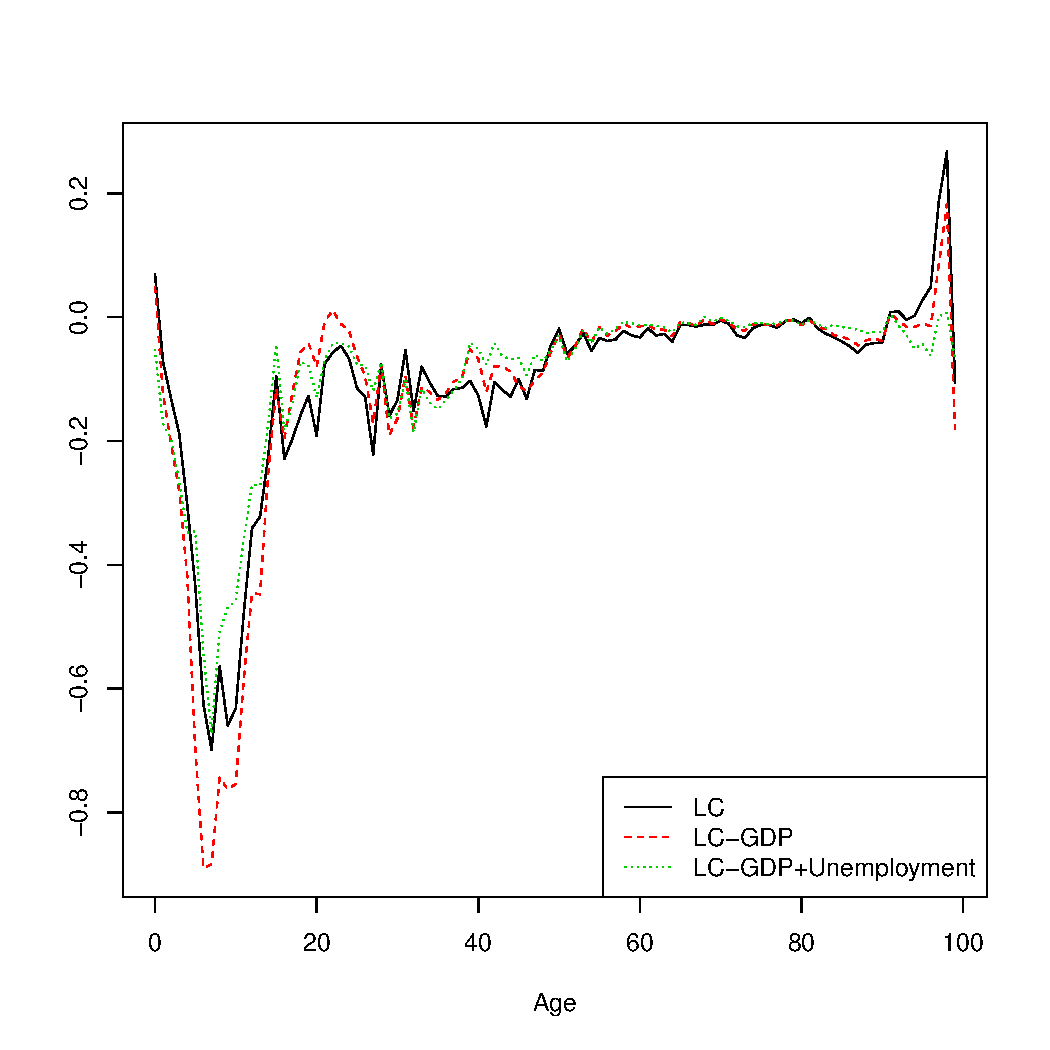
\includegraphics[width=\linewidth]{CAN_error_age_male} 
		\caption{Mean Error over Time}
		\label{fig:errora}
	\end{subfigure}
	\begin{subfigure}{0.4\textwidth}
		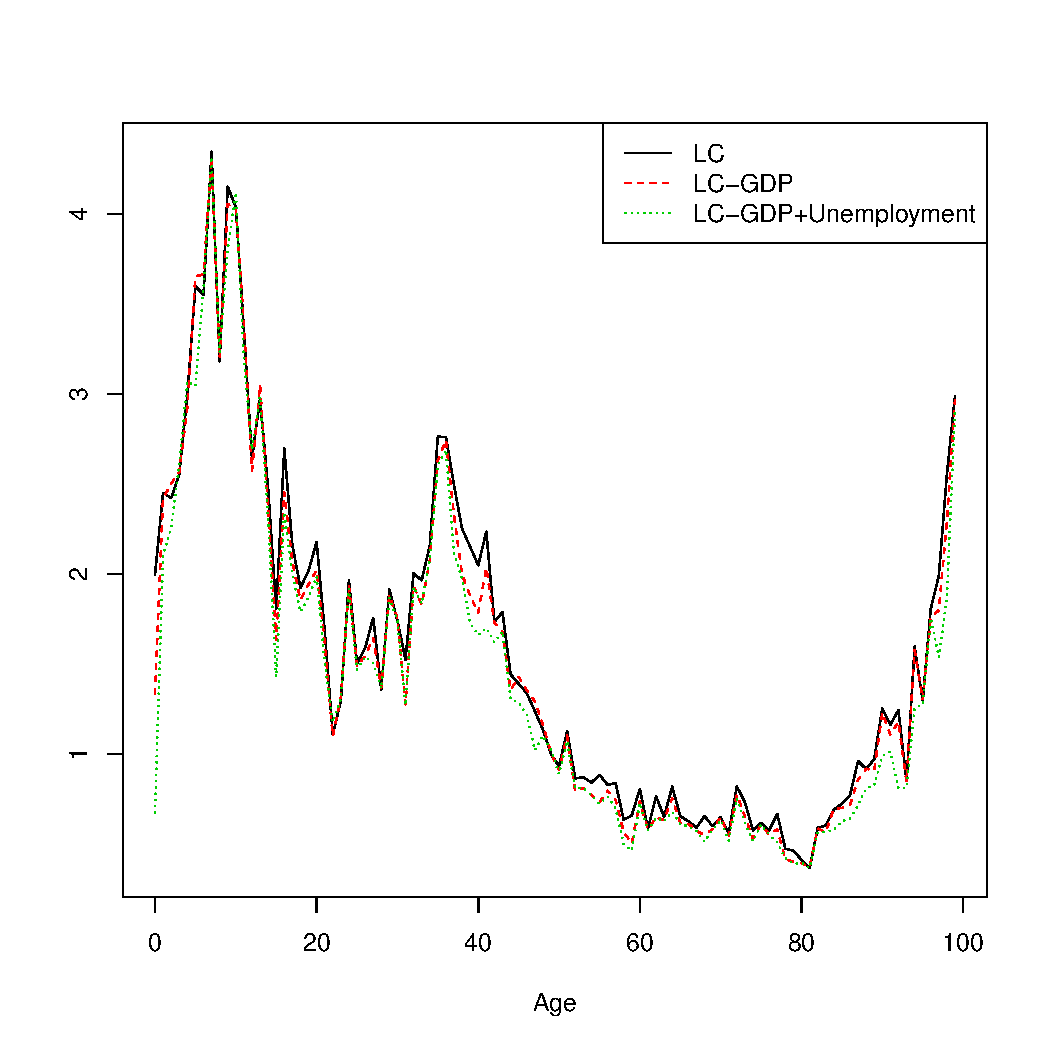
\includegraphics[width=\linewidth]{CAN_abs_error_age_male} 
		\caption{Mean Absolute Error over Time}
		\label{fig:errorb}
	\end{subfigure}
	\begin{subfigure}{0.4\textwidth}
		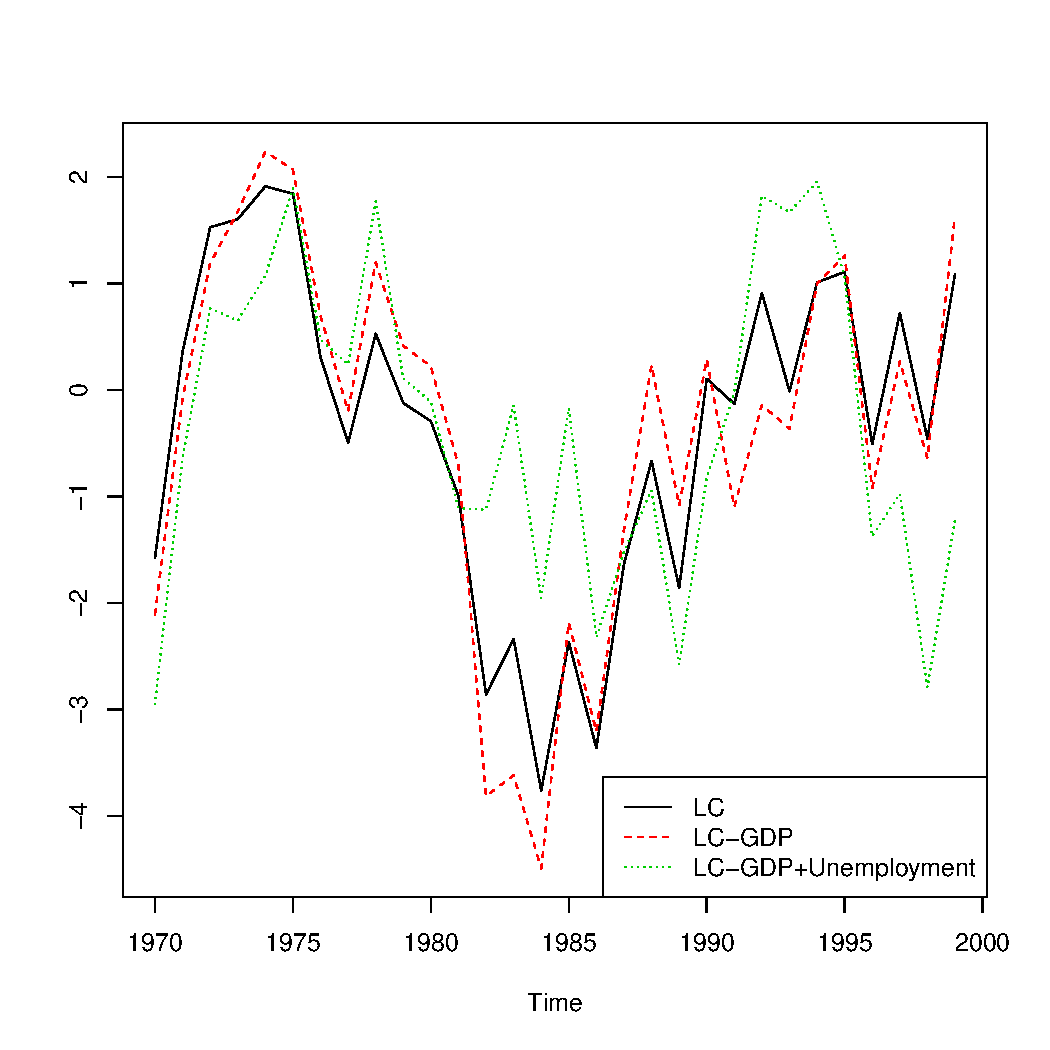
\includegraphics[width=\linewidth]{CAN_error_time_male} 
		\caption{Mean Error over Age}
		\label{fig:errorc}
	\end{subfigure}
	\begin{subfigure}{0.4\textwidth}
		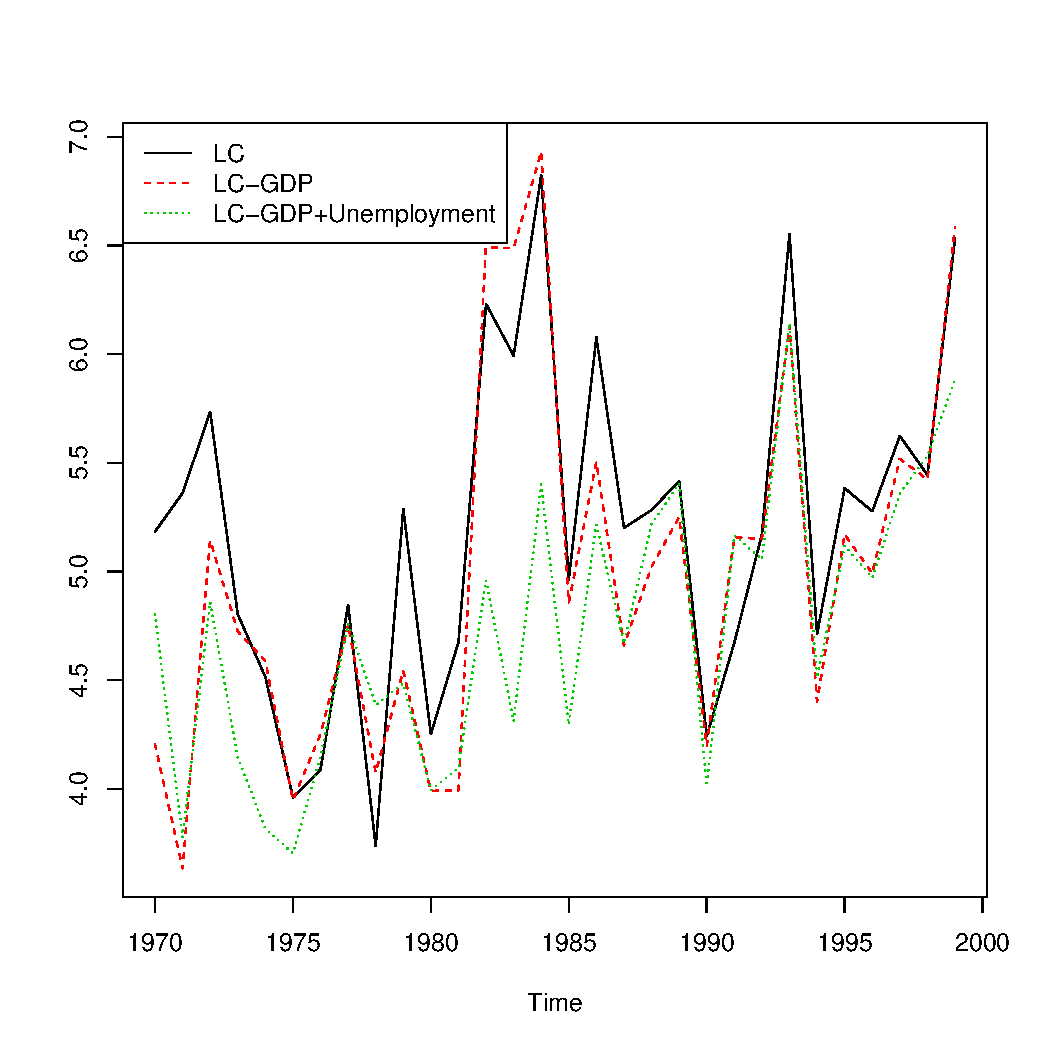
\includegraphics[width=\linewidth]{CAN_abs_error_time_male} 
		\caption{Mean Absolute Error over Age}
		\label{fig:errord}
	\end{subfigure}
	\caption{Mean error for $\ln(\mu_{xt})$ for Canadian males}
\end{figure}

In final representation of the goodness-of-fit of our models, we plotted the fitted errors given by 
\begin{align}
	\hat{\epsilon} = \ln\mu_{xt}-\ln\hat{\mu}_{xt}
\end{align}
where $\ln\hat{\mu}_{xt}$ is the estimated log mortality rates and $\ln\mu_{xt}$ is the actual log mortality rates.

Figure \ref{fig:errora} and Figure \ref{fig:errorb} show the mean errors and mean absolute errors averaged out over time, i.e. $\frac{1}{T} \sum_t (\ln\mu_{xt}-\ln\hat{\mu}_{xt})$ and $\frac{1}{T} \sum_t |\ln\mu_{xt}-\ln\hat{\mu}_{xt}|$. This seems to indicate that all three models do not fit well for particularly low or high values of $x$.  Figure \ref{fig:errorc} and Figure \ref{fig:errord} show the mean errors and mean absolute errors averaged out over age, i.e. $\frac{1}{X} \sum_x (\ln\mu_{xt}-\ln\hat{\mu}_{xt})$ and $\frac{1}{X} \sum_x |\ln\mu_{xt}-\ln\hat{\mu}_{xt}|$. And for errors averaged out over age, we don't see any particular clear trends in time. Note that Figure 5, given in the appendix, shows the exact same results for females.


\subsection{Out-of-Sample test}

After having estimated the model on a subsample of the data, i.e. from 1970 to 1999, we forecast the mortality rates for the years 2000 to 2009 and compared the predicted values to the real values from the dataset. To forecast $\kappa_t$ we fitted the best ARIMA$(p,d,q)$ model according to the AIC. For $g_t$ only, we used the same approach by finding the best ARIMA$(p,d,q)$ model again according to the AIC. For both $g_t$ and $u_t$, we use a VAR$(p)$ model where $p$ is selected according to the AIC. Note that for both males and females, we find that $p=2$ gave the best fit.

Figure \ref{fig:prederrora} and Figure \ref{fig:prederrorb} show the mean forecast errors and mean absolute forecast errors averaged out over time, while Figure \ref{fig:prederrorc} and Figure \ref{fig:prederrord} show the mean forecast errors and mean absolute forecast errors averaged out over age.

\begin{figure}[!htp]
	\begin{subfigure}{0.4\textwidth}
		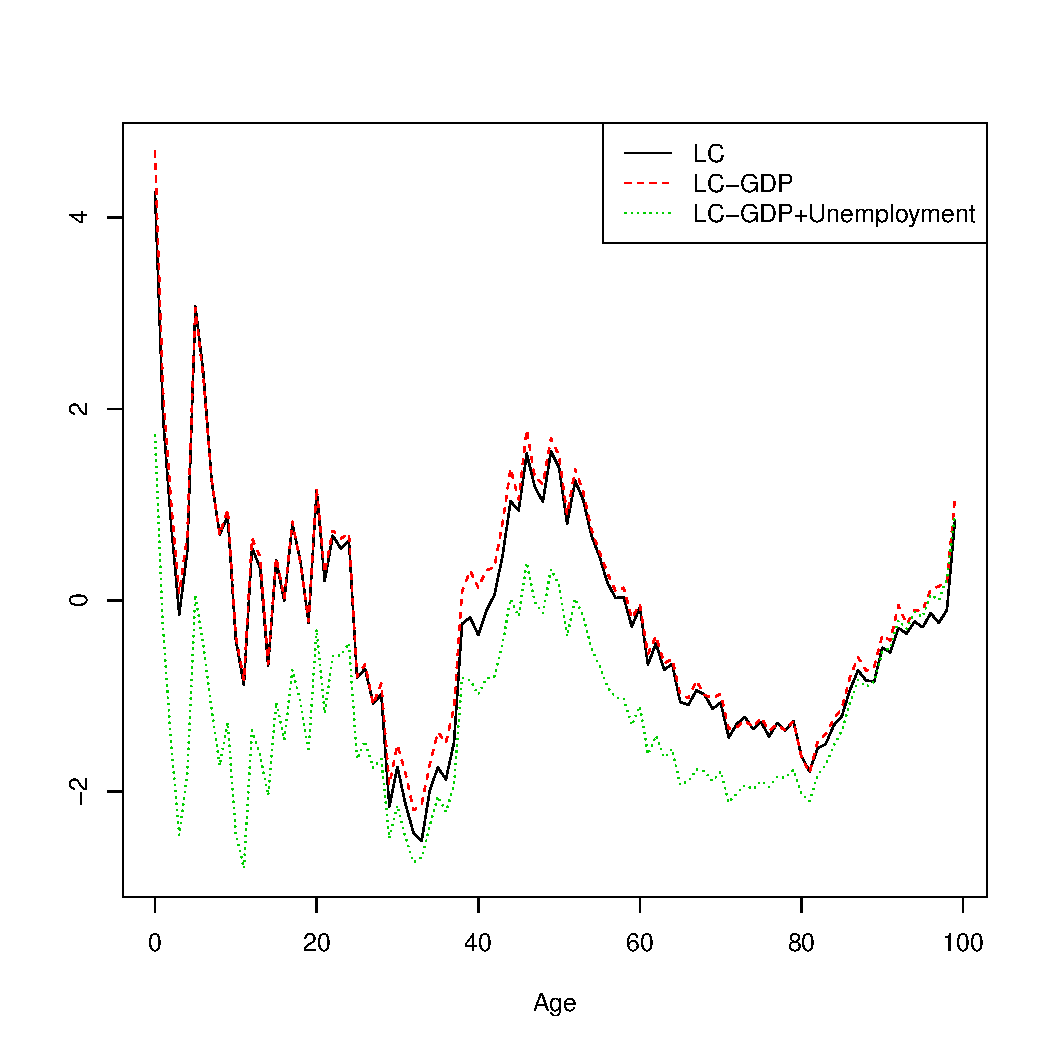
\includegraphics[width=\linewidth]{CAN_pred_error_age_male} 
		\caption{Mean Error over Time}
		\label{fig:prederrora}
	\end{subfigure}
	\begin{subfigure}{0.4\textwidth}
		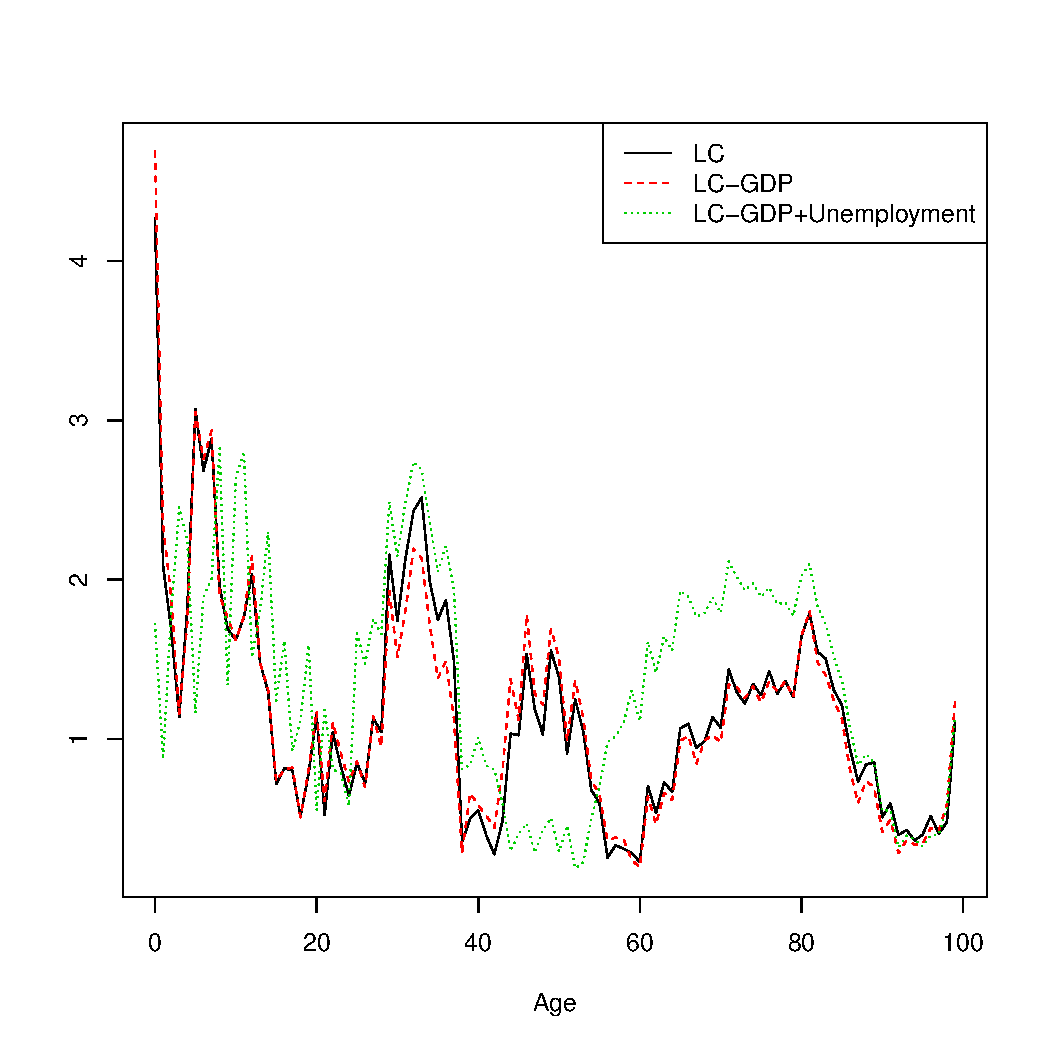
\includegraphics[width=\linewidth]{CAN_abs_pred_error_age_male} 
		\caption{Mean Absolute Error over Time}
		\label{fig:prederrorb}
	\end{subfigure}
	\begin{subfigure}{0.4\textwidth}
		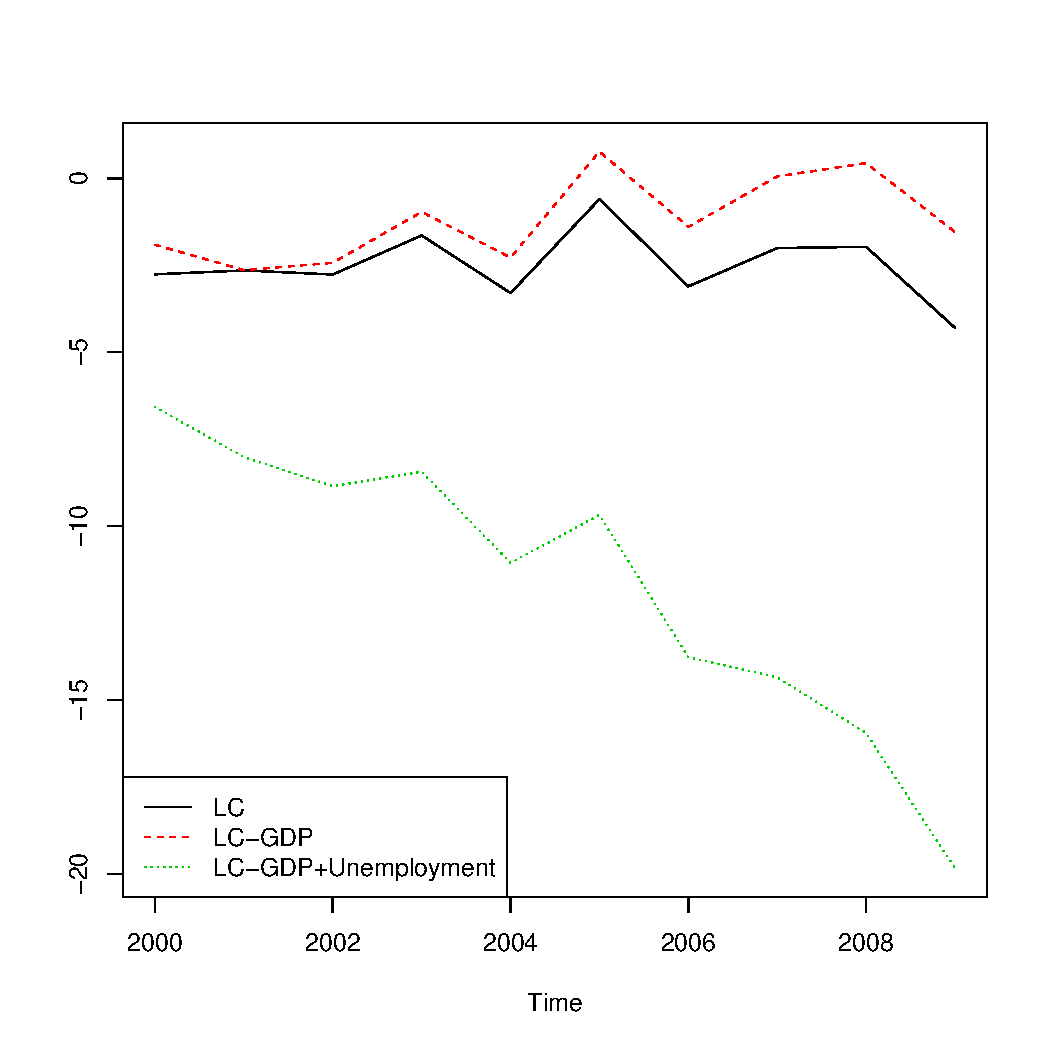
\includegraphics[width=\linewidth]{CAN_pred_error_time_male} 
		\caption{Mean Error over Age}
		\label{fig:prederrorc}
	\end{subfigure}
	\begin{subfigure}{0.4\textwidth}
		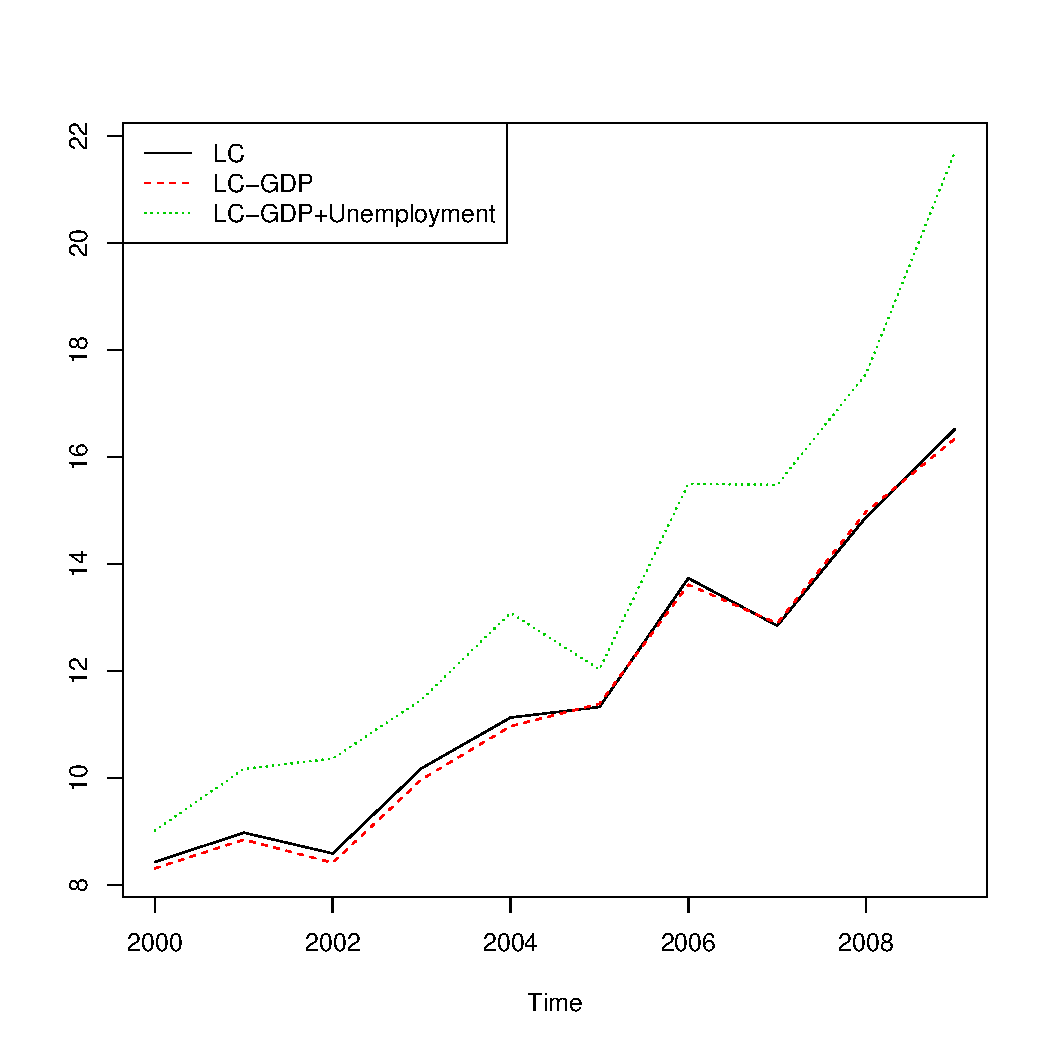
\includegraphics[width=\linewidth]{CAN_abs_pred_error_time_male} 
		\caption{Mean Absolute Error over Age}
		\label{fig:prederrord}
	\end{subfigure}
	\caption{Mean error for $\ln(\mu_{xt})$ for Canadian males}
\end{figure}

If we look at Figure \ref{fig:prederrorc} and Figure \ref{fig:prederrord}, we see that over time the forecast errors become bigger as expected, but that when including only GDP as a covariate we get a slightly better forecast than either the traditional model or the one with GDP and unemployment. This is only true for Canadian males as Figure 6 shows that for female, both model with covariates performed worst than the model with no covariates.

In order to quantify and compare these deviations of the forecast log mortality rates from the actual log mortality rates, we computed the root forecast mean squared errors (RFMSE) for every model. The RFMSE is given by the following formula
\begin{align}
RFMSE = \frac{1}{X}\frac{1}{T_f}\sum_x \sum_t (\ln\mu_{xt}-\ln\tilde{\mu}_{xt})^2
\end{align}
where $\tilde{\mu}_{xt}$ is the forecast for the log mortality rates and $T_f$ is the number of forecast time periods. Results are reported in Table \ref{teb:rmsfe}.

\begin{table}[!htp]
	\centering
	\caption{Out-of-sample Results: Root forecast mean squared errors}
	\label{teb:rmsfe}
	\begin{tabular}{lll}
		\hline
		Model                                                              & Male    & Female   \\ \hline
		$\alpha_x + \beta_x \kappa_t$                                      & 0.15266 & 0.13429* \\
		$\alpha_x + \beta_x \kappa_t + \gamma_{1x} g_t$                    & 0.15264* & 0.15096 \\
		$ \alpha_x + \beta_x \kappa_t + \gamma_{1x} g_t + \gamma_{2x} u_t$ & 0.17550 & 0.16860 \\ \hline
	\end{tabular}
\end{table}

As predicted by looking at Figure 3 and Figure 6,  the original model performs better for forecasting mortality rates for females, while the model with only GDP as a covariate performs just a bit better for males. While \cite{Niu2014} found that the model with GDP performed better in every setting compared to the original model, we do not share the same conclusion here. One possible explanation is that our dataset is smaller (1970 to 1999 compared to 1950 to 1999) and we forecast on a longer period (2000 to 2009 compared to 2000 to 2007). In addition, \cite{Niu2014} used the original \cite{Lee1992} model, while we used the extension proposed by \cite{Brouhns2002}. Moreover, if we changed our forecasting approach for $g_t$ and $u_t$, we could get different results. 


\section{Conclusion} \label{sec:conclusion}

In this paper, we estimated and proposed an extension the \cite{Brouhns2002} model of mortality rates by including covariates. Based on Canadian data from 1970 to 2009 for mortality, GDP and unemployment, we found inconclusive evidence for the systematic inclusion of covariates in the \cite{Brouhns2002} model. Both out-of-sample tests and in-sample tests gave conflicting evidence to whether we should systematically include covariates or not. In fact, it does not seem like including covariates really worsen or better the fit by a big factor.

And while our results seem to defy the purpose of the our paper, we want to stress to the reader that the our approach is simply meant as a gateway to bridge the gap between extrapolative and explicative models in the literature. Additionally, the idea of integrating socio-economic variables in the model is not solely to better forecast, but to also better interpret the role of these variables on mortality rates. Furthermore, as mentioned previously, we only used a VAR$(p)$ model to predict GDP and unemployment. The fact is that better and more sophisticated model could be use which might greatly improve the fit of our model.

Hence, to further understand the role of socio-economic variables in mortality rates, we propose to extend this research to bigger datasets, i.e. more years to be included in the calibration of the model, and more countries. Moreover, it could interesting to see how other observable factors such as investment in medical research,  environmental factors, and etc. could impact our model. 

Finally, while the model we propose is quite general, its real strength lies in the fact that it can be extend easily. For example, one could effortlessly expand on this model by writing it in terms of the more general linear model framework. Thankfully, as we live longer, we will have more time to further our understanding of this topic.

\bibliographystyle{aea}
\bibliography{mendeley}

\clearpage

\section{Appendix}

\subsection{Proof of Theorem \ref{the:1}}
\textit{Proof.}

\begin{enumerate}
	\item[(i)] For any $\theta$ we can construct $\theta^o$ by using \ref{eq:par_1} and letting $ d = \sum_{x=1}^{X} \beta_x$, $ c = - \frac{\sum_{t=1}^{T} \kappa_t}{T}$, and $e = \frac{cov(\kappa_t, g_t)}{var(g_t)}$
	\item[(ii)] One can transform $\theta^o$ into the original $\theta$ by $d^o = \frac{1}{d}$, $c^o = -cd$, and $e^o = -ed$. The parametrization \ref{eq:par_1} is invariant to $c$, $d$, $e$.
	\item[(iii)] Consider $\theta_1 \neq \theta_2$
	\begin{enumerate}
		\item [\textbf{Step 1}] If $\alpha_x^1 \neq \alpha_x^2$ for some $x$ then $\frac{1}{T} \sum_{t=1}^{T} m_{xt}^1 = \alpha_x^1 \neq \alpha_x^2 = \sum_{t=1}^{T} m_{xt}^2$
		\item [\textbf{Step 2}] If $\gamma_x^1 \neq \gamma_x^2$ for some $x$ then, since $cov(\kappa_t, g_t)=0$, it holds $cov(g_t, m_{xt}^1)= \gamma_x^1 var(g_t) \neq \gamma_x^2 var(g_t) = cov(g_t, m_{xt}^2)$
		\item [\textbf{Step 3}] If $\alpha_x^1=\alpha_x^2$ and $\gamma_x^1=\gamma_x^2$ for all $x$, but $\kappa_t^1 \neq \kappa_t^2$ for some $t$, then, since $\sum_{x=1}^{X} \beta_x =1$, it holds
		\begin{align*}
			\sum_{x=1}^{X}m_{xt}^1 = \kappa_x^1 - \sum_{x=1}^{X} \alpha_x^1 - \sum_{x=1}^X \gamma_x^1 g_t \neq \kappa_x^2 - \sum_{x=1}^{X} \alpha_x^2 - \sum_{x=1}^X \gamma_x^2 g_t = \sum_{x=1}^{X}m_{xt}^2 
		\end{align*}
		\item [\textbf{Step 4}] If $\alpha_x^1=\alpha_x^2$ and $\gamma_x^1=\gamma_x^2$ for all $x$, but $\kappa_t^1 = \kappa_t^2$ for all $t$, and $\kappa \neq 0$, but $\beta_x^1 \neq \beta_x^2$ for some $x$, then we can find $\kappa_{t_1}^2 = \kappa_{t_1}^1 \neq \kappa_{t_2}^1 = \kappa_{t_2}^2$, such that $m_{xt_2}^1- m_{xt_1}^1 = \beta_x^1 (\kappa_{t_2}^1-\kappa_{t_1}^1) \neq (\kappa_{t_2}^2-\kappa_{t_1}^2) = m_{xt_2}^2- m_{xt_1}^2$
	\end{enumerate}
\end{enumerate}

\subsection{Proof of Theorem \ref{the:2}}
\textit{Proof.}

\begin{enumerate}
	\item[(i)] For any $\theta$ we can construct $\theta^o$ by using \ref{eq:par_1} and letting $ d = \sum_{x=1}^{X} \beta_x$, $ c = - \frac{\sum_{t=1}^{T} \kappa_t}{T}$, and $e = \frac{cov(\kappa_t, Y'_t)}{var(Y'_t)}$
	\item[(ii)] One can transform $\theta^o$ into the original $\theta$ by $d^o = \frac{1}{d}$, $c^o = -cd$, and $e^o = -ed$. The parametrization \ref{eq:par_1} is invariant to $c$, $d$, $e$.
	\item[(iii)] Consider $\theta_1 \neq \theta_2$
	\begin{enumerate}
		\item [\textbf{Step 1}] If $\alpha_x^1 \neq \alpha_x^2$ for some $x$ then $\frac{1}{T} \sum_{t=1}^{T} m_{xt}^1 = \alpha_x^1 \neq \alpha_x^2 = \sum_{t=1}^{T} m_{xt}^2$
		\item [\textbf{Step 2}] If $\gamma_x^1 \neq \gamma_x^2$ for some $x$ then, since $cov(\kappa_t, Y'_t)=0$, it holds $cov(Y'_t, m_{xt}^1)= \gamma_x^1 var(Y'_t) \neq \gamma_x^2 var(Y'_t) = cov(Y'_t, m_{xt}^2)$
		\item [\textbf{Step 3}] If $\alpha_x^1=\alpha_x^2$ and $\gamma_x^1=\gamma_x^2$ for all $x$, but $\kappa_t^1 \neq \kappa_t^2$ for some $t$, then, since $\sum_{x=1}^{X} \beta_x =1$, it holds
		\begin{align*}
		\sum_{x=1}^{X}m_{xt}^1 = \kappa_x^1 - \sum_{x=1}^{X} \alpha_x^1 - \sum_{x=1}^X \gamma_x^1 Y'_t \neq \kappa_x^2 - \sum_{x=1}^{X} \alpha_x^2 - \sum_{x=1}^X \gamma_x^2 Y'_t = \sum_{x=1}^{X}m_{xt}^2 
		\end{align*}
		\item [\textbf{Step 4}] If $\alpha_x^1=\alpha_x^2$ and $\gamma_x^1=\gamma_x^2$ for all $x$, but $\kappa_t^1 = \kappa_t^2$ for all $t$, and $\kappa \neq 0$, but $\beta_x^1 \neq \beta_x^2$ for some $x$, then we can find $\kappa_{t_1}^2 = \kappa_{t_1}^1 \neq \kappa_{t_2}^1 = \kappa_{t_2}^2$, such that $m_{xt_2}^1- m_{xt_1}^1 = \beta_x^1 (\kappa_{t_2}^1-\kappa_{t_1}^1) \neq (\kappa_{t_2}^2-\kappa_{t_1}^2) = m_{xt_2}^2- m_{xt_1}^2$
	\end{enumerate}
\end{enumerate}

\begin{figure}[!htp]
	\begin{subfigure}{0.4\textwidth}
		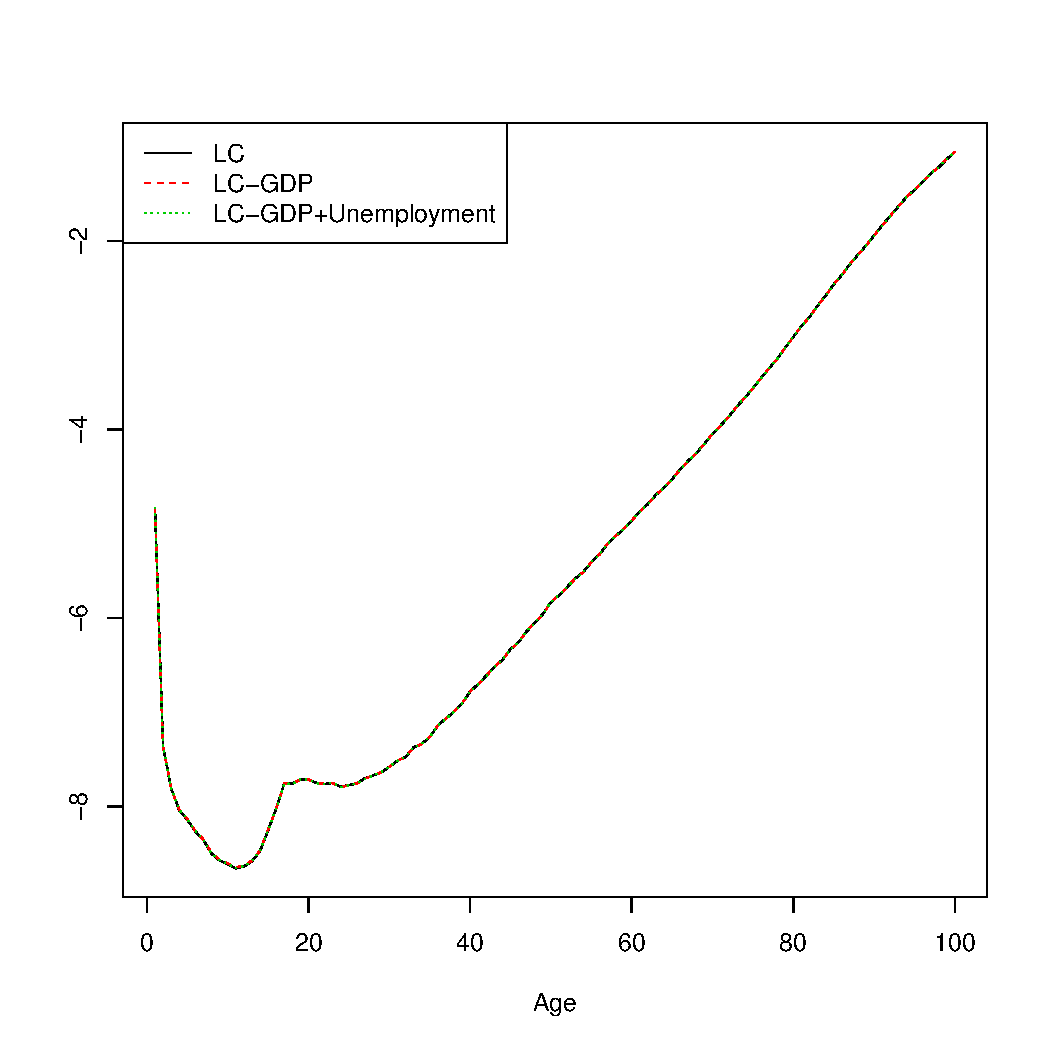
\includegraphics[width=\linewidth]{CAN_ax_female}
		\caption{$\alpha_x$}
		\label{fig:femalea}
	\end{subfigure}
	\begin{subfigure}{0.4\textwidth}
		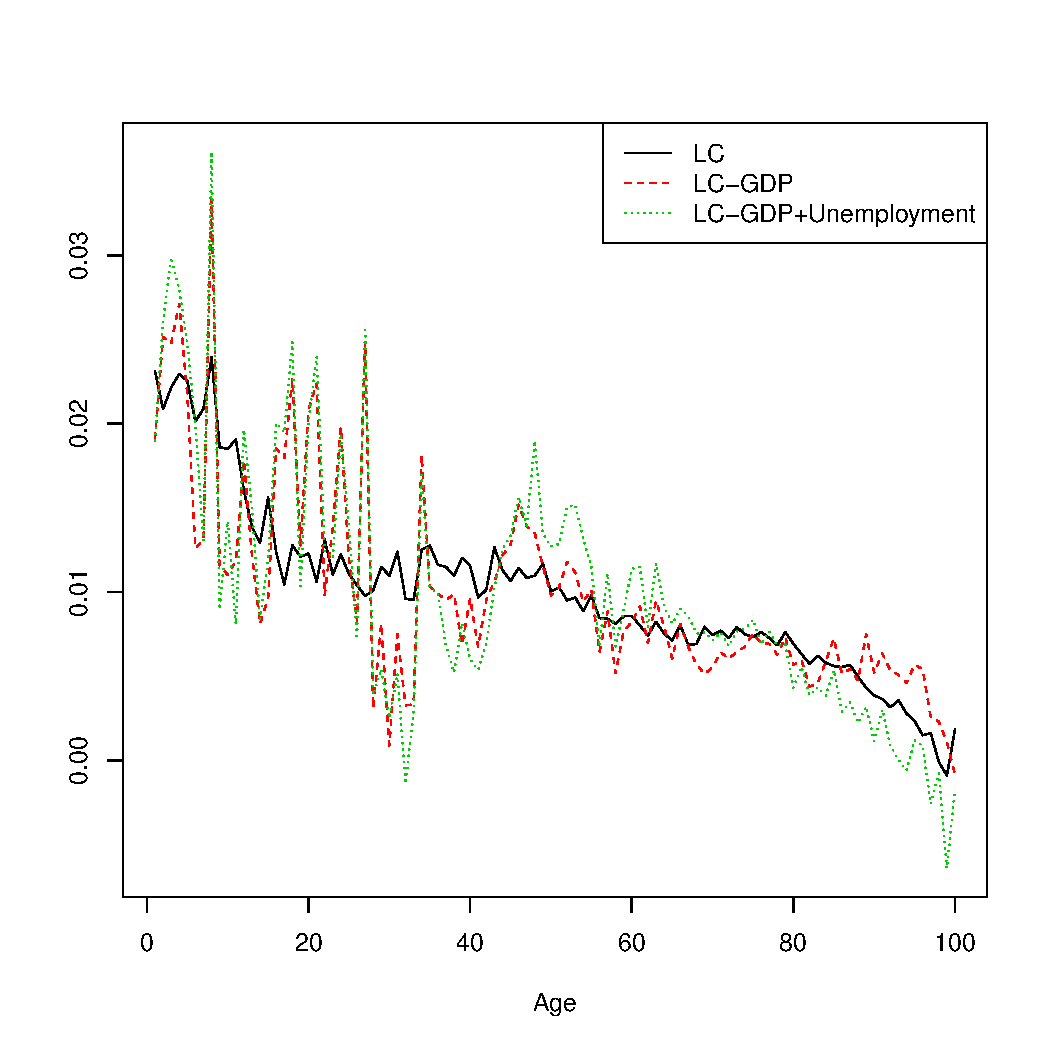
\includegraphics[width=\linewidth]{CAN_bx_female}
		\caption{$\beta_x$}
		\label{fig:femaleb}  
	\end{subfigure}
	\begin{subfigure}{0.4\textwidth}
		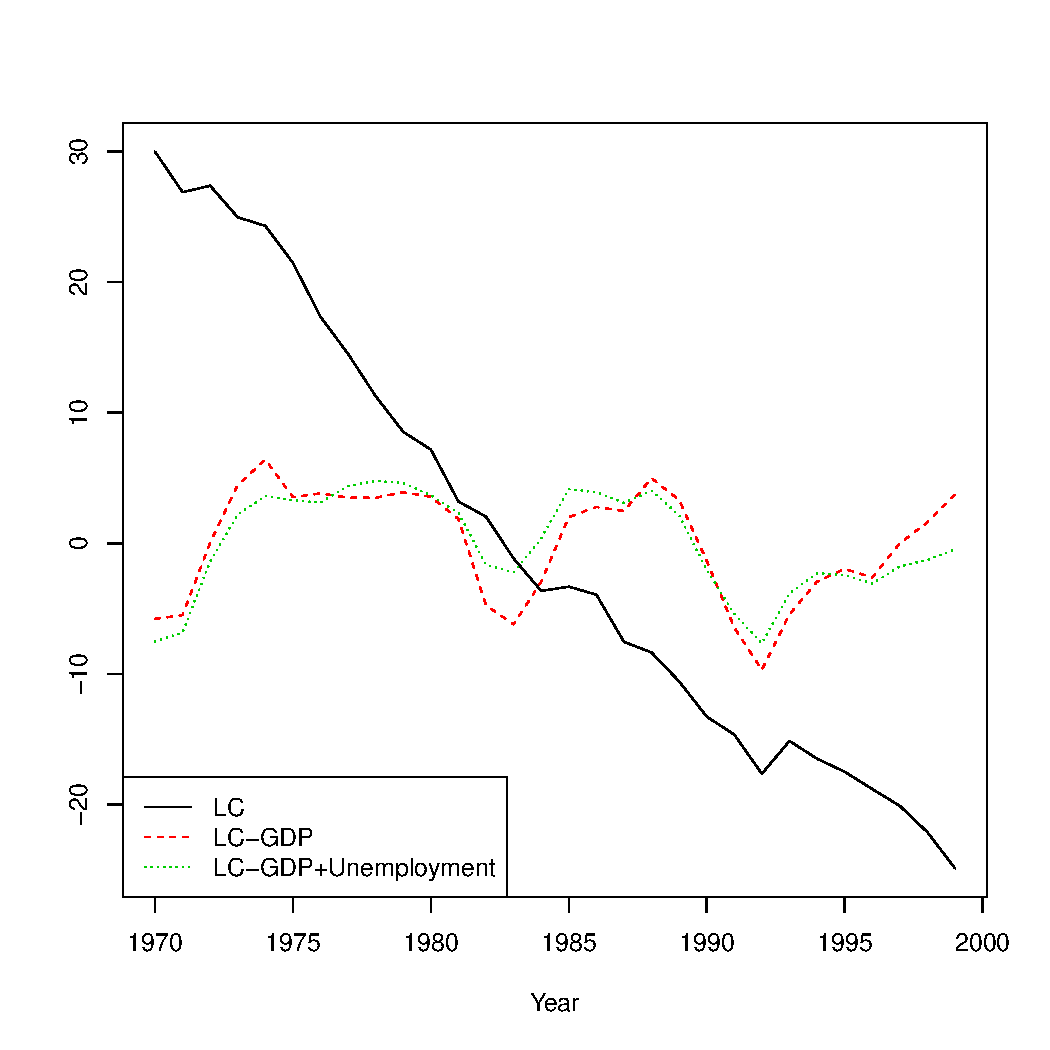
\includegraphics[width=\linewidth]{CAN_kt_female}
		\caption{$\kappa_t$}
		\label{fig:femalec} 
	\end{subfigure}
	\begin{subfigure}{0.4\textwidth}
		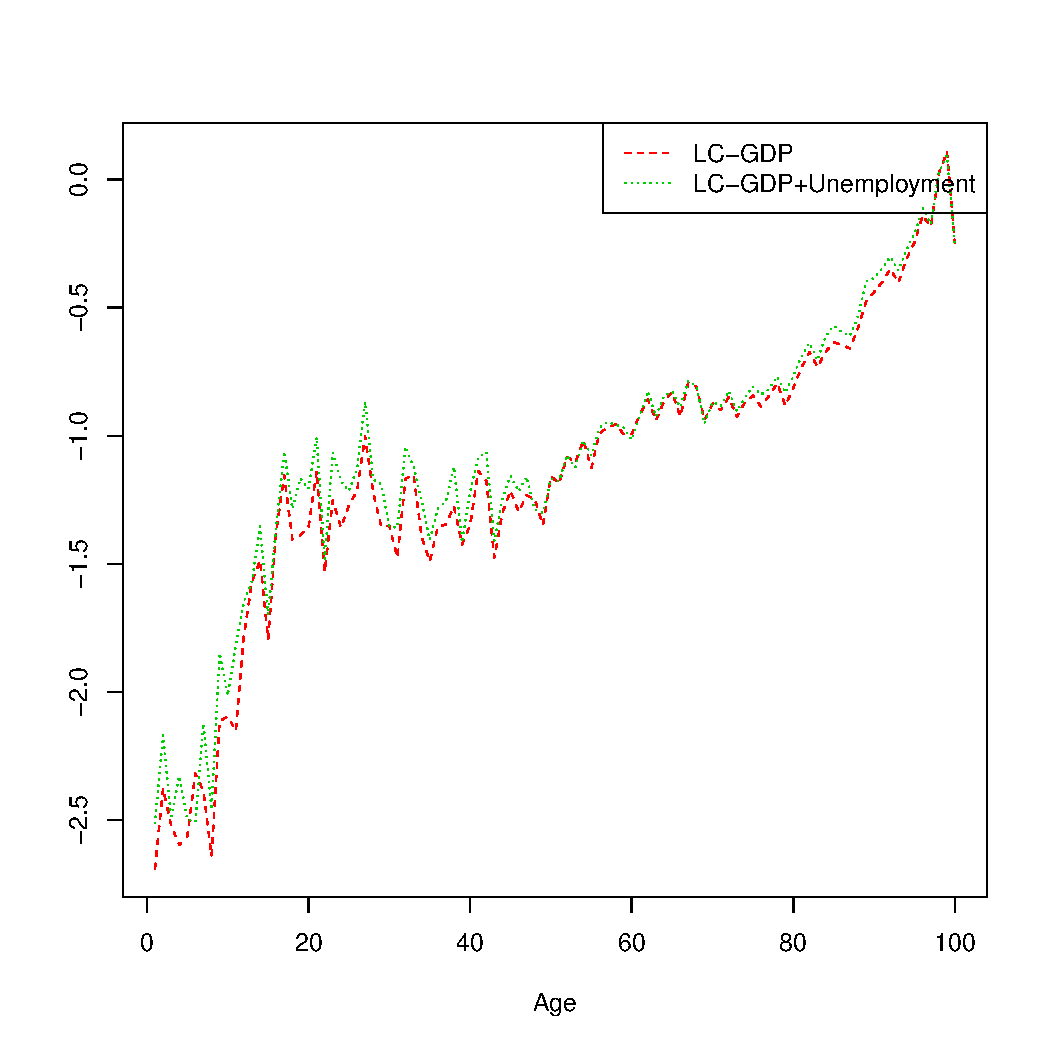
\includegraphics[width=\linewidth]{CAN_g1x_female}
		\caption{$\gamma_{x,gdp}$}
		\label{fig:femaled} 
	\end{subfigure}
	\begin{subfigure}{0.4\textwidth}
		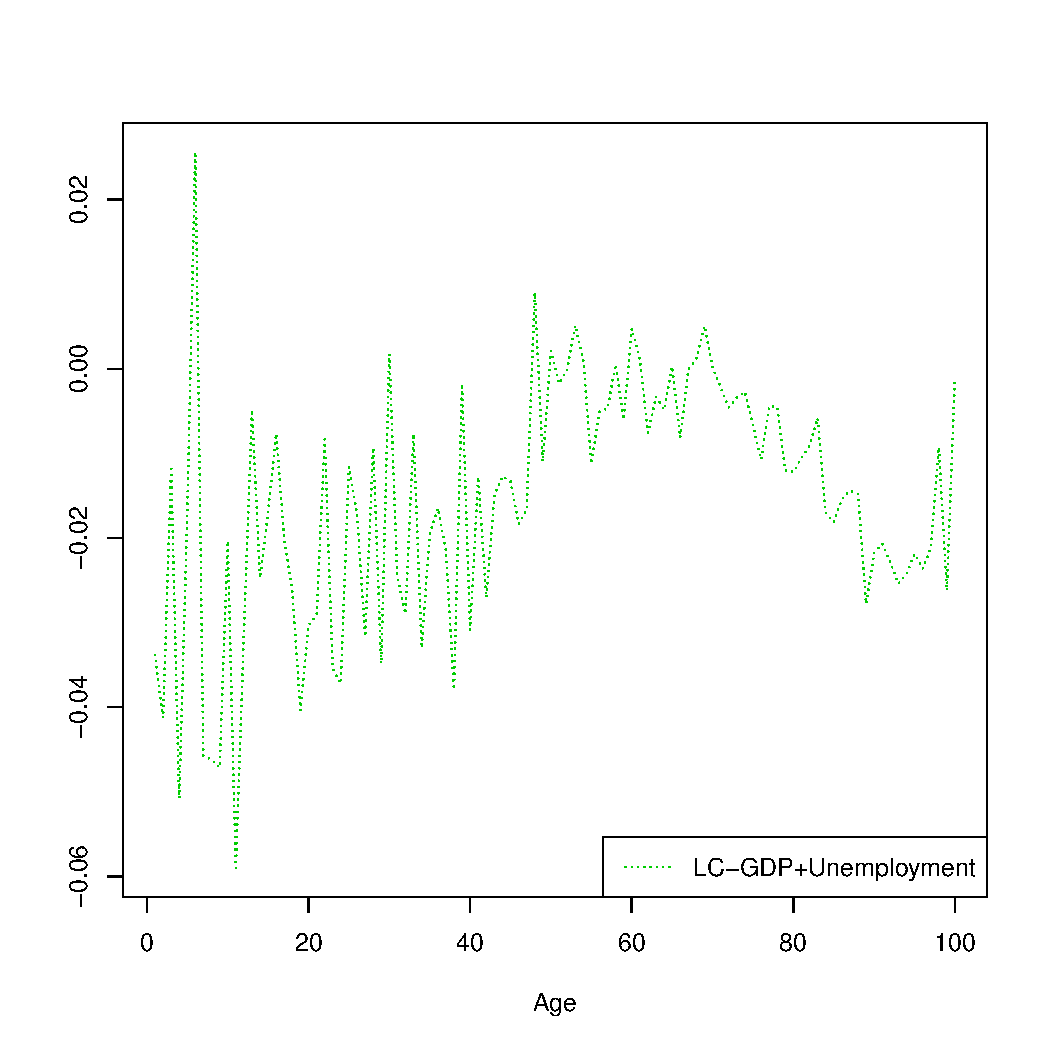
\includegraphics[width=\linewidth]{CAN_g2x_female} 
		\caption{$\gamma_{x,unemployment}$}
		\label{fig:femalee} 
	\end{subfigure}
	\caption{Poisson log-bilinear extension with covariates for Canadian females}
\end{figure}

\begin{figure}[!htp]
	\begin{subfigure}{0.4\textwidth}
		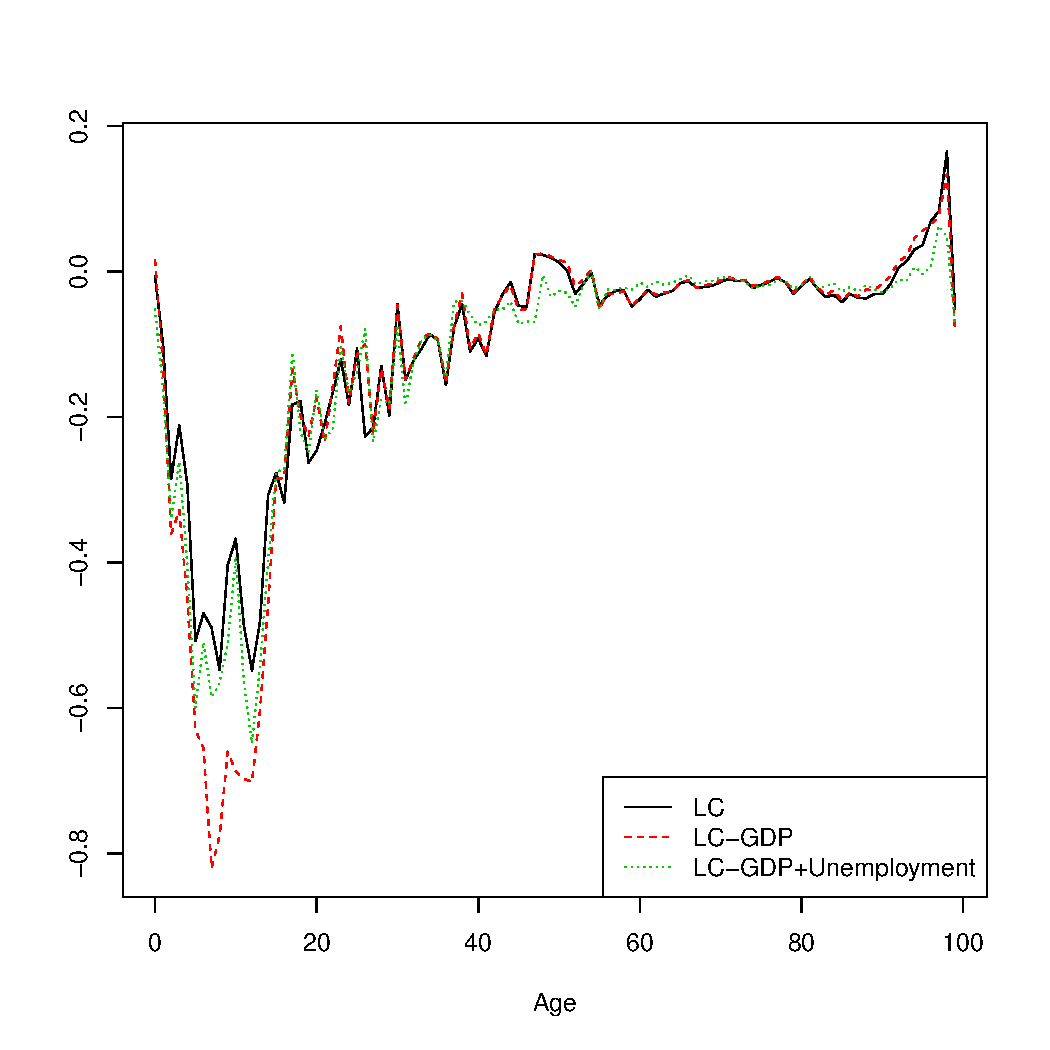
\includegraphics[width=\linewidth]{CAN_error_age_female} 
		\caption{Mean Error over Time}
	\end{subfigure}
	\begin{subfigure}{0.4\textwidth}
		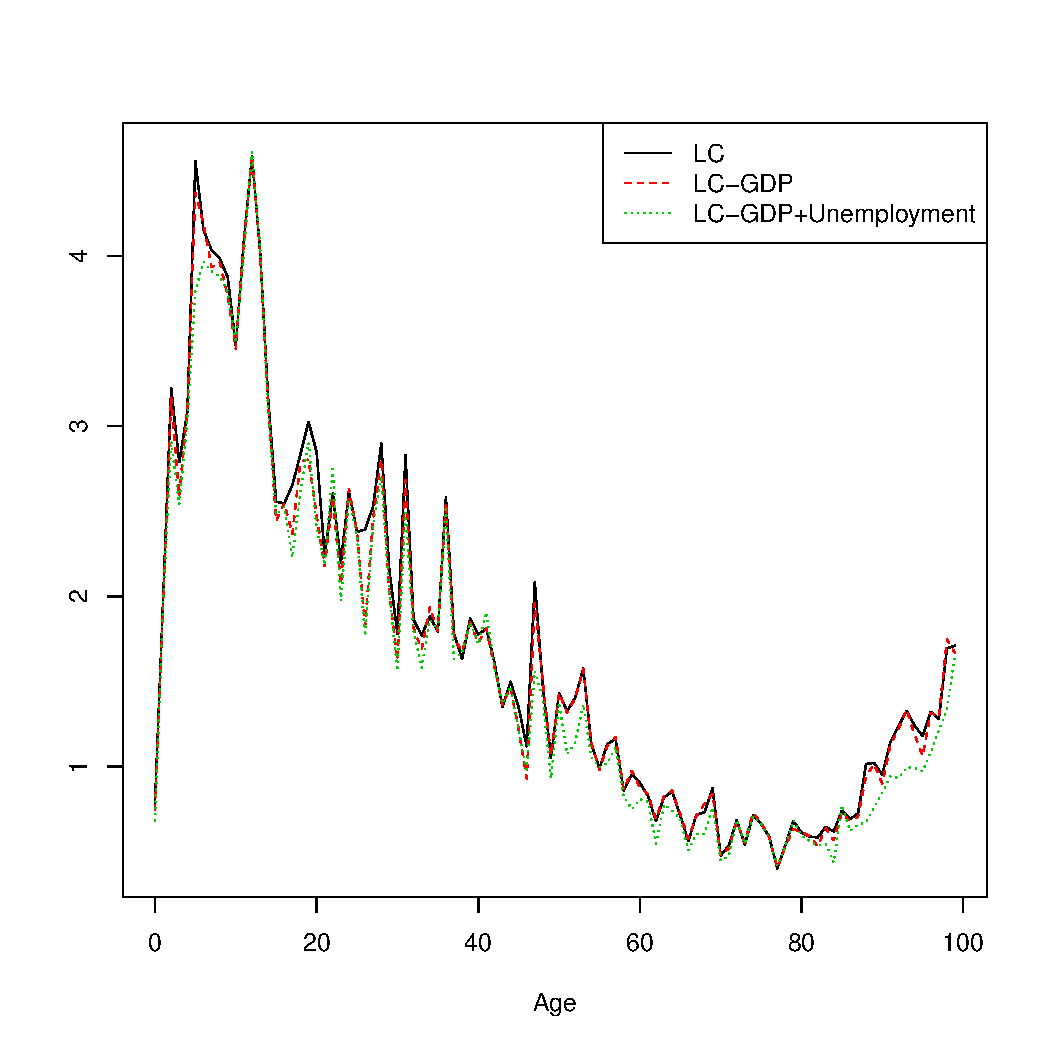
\includegraphics[width=\linewidth]{CAN_abs_error_age_female} 
		\caption{Mean Absolute Error over Time}
	\end{subfigure}
	\begin{subfigure}{0.4\textwidth}
		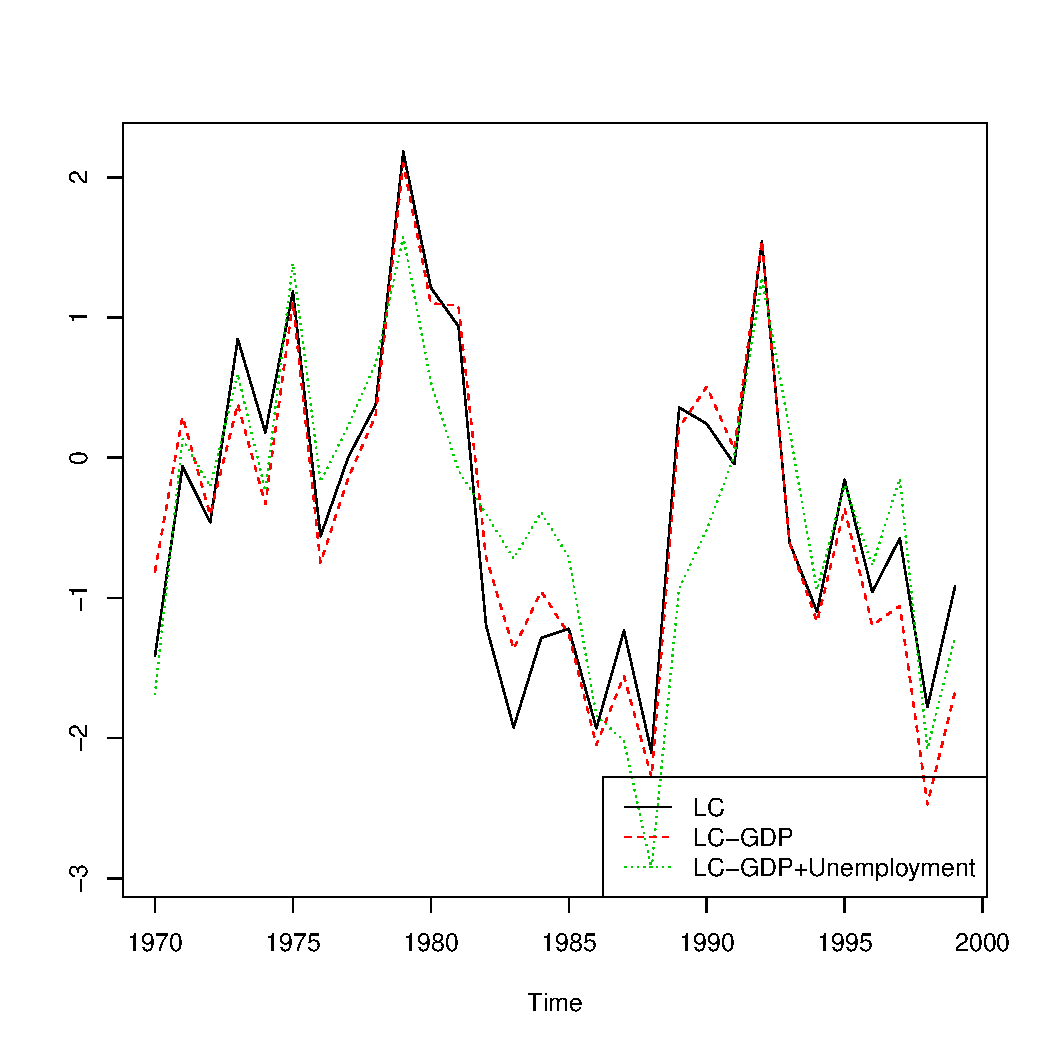
\includegraphics[width=\linewidth]{CAN_error_time_female} 
		\caption{Mean Error over Age}
	\end{subfigure}
	\begin{subfigure}{0.4\textwidth}
		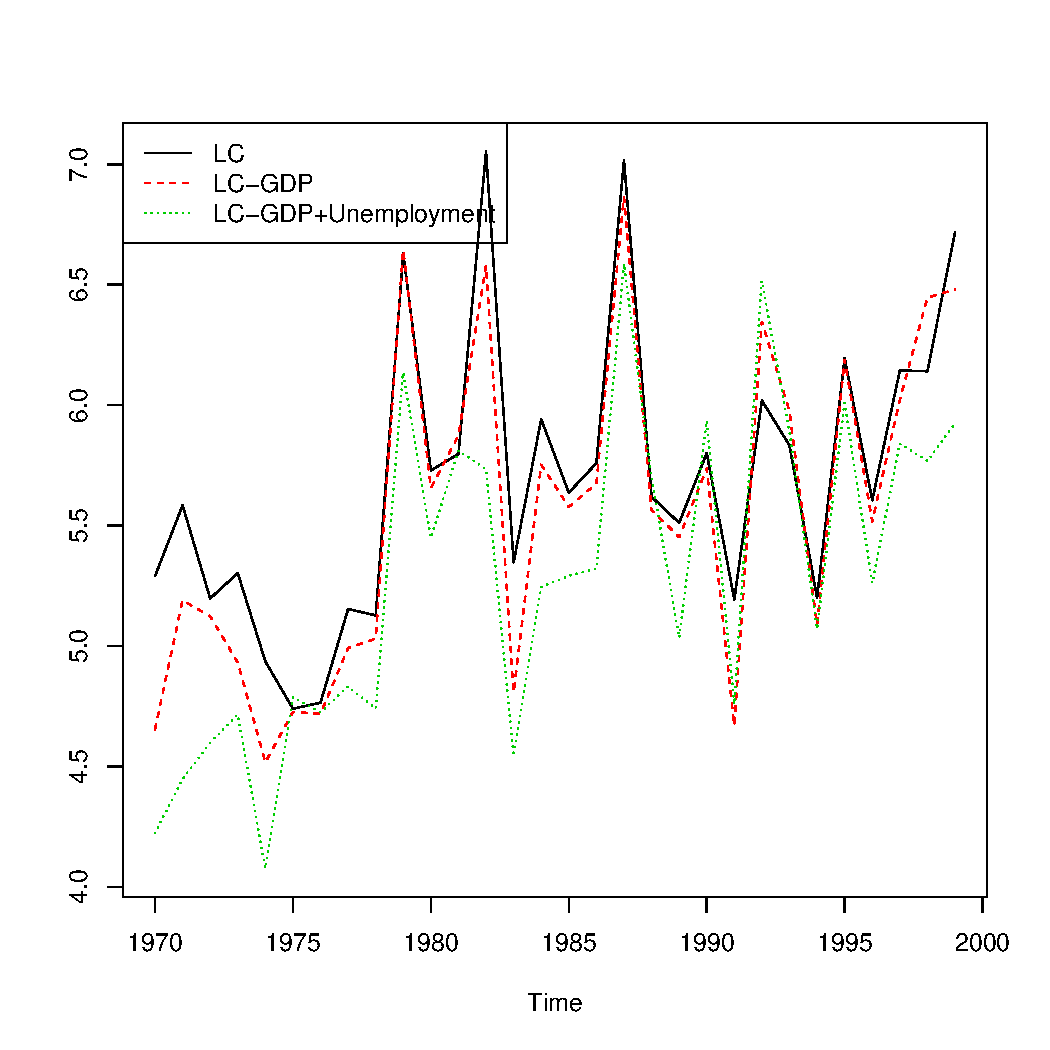
\includegraphics[width=\linewidth]{CAN_abs_error_time_female} 
		\caption{Mean Absolute Error over Age}
	\end{subfigure}
	\caption{Mean error for $\ln(\mu_{xt})$ for Canadian females}
\end{figure}

\begin{figure}[!htp]
	\begin{subfigure}{0.4\textwidth}
		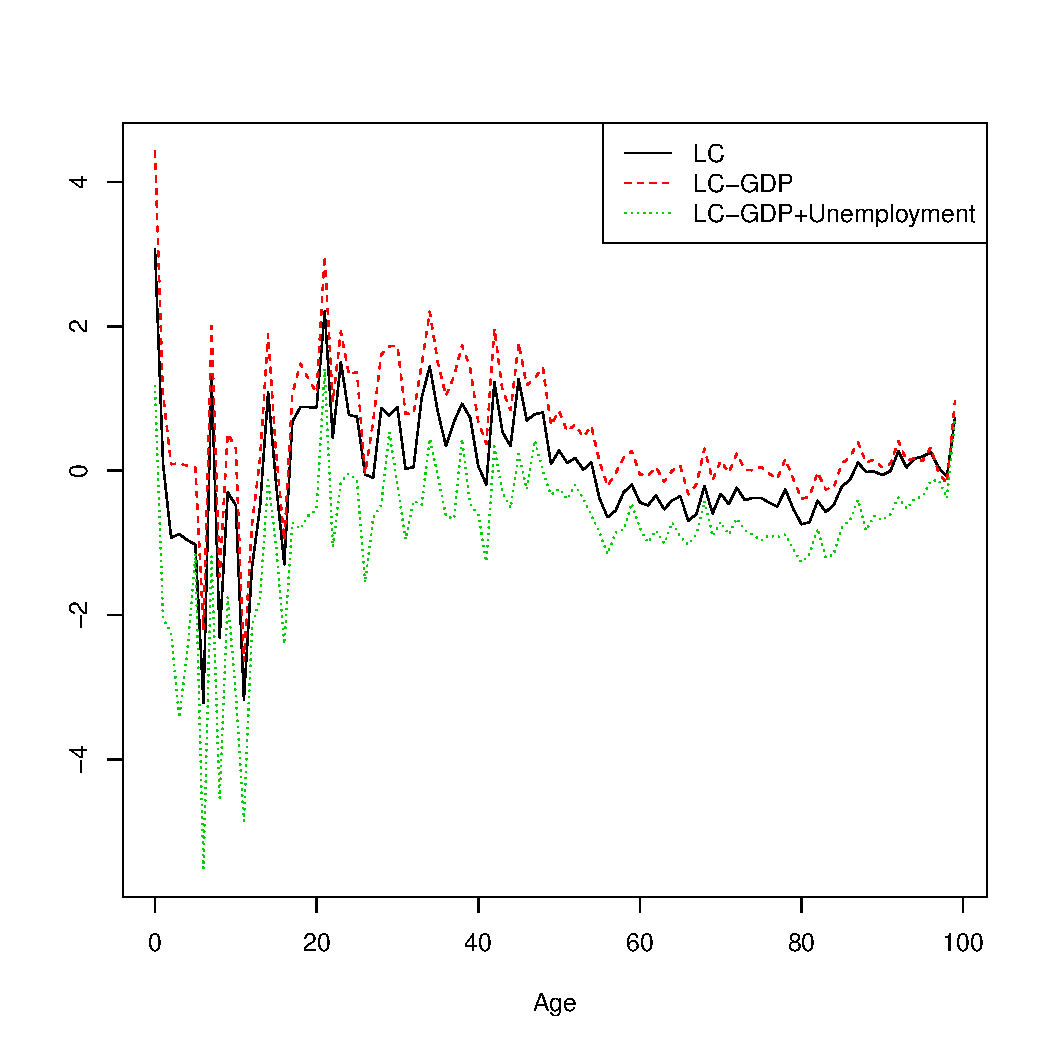
\includegraphics[width=\linewidth]{CAN_pred_error_age_female} 
		\caption{Mean Error over Time}
	\end{subfigure}
	\begin{subfigure}{0.4\textwidth}
		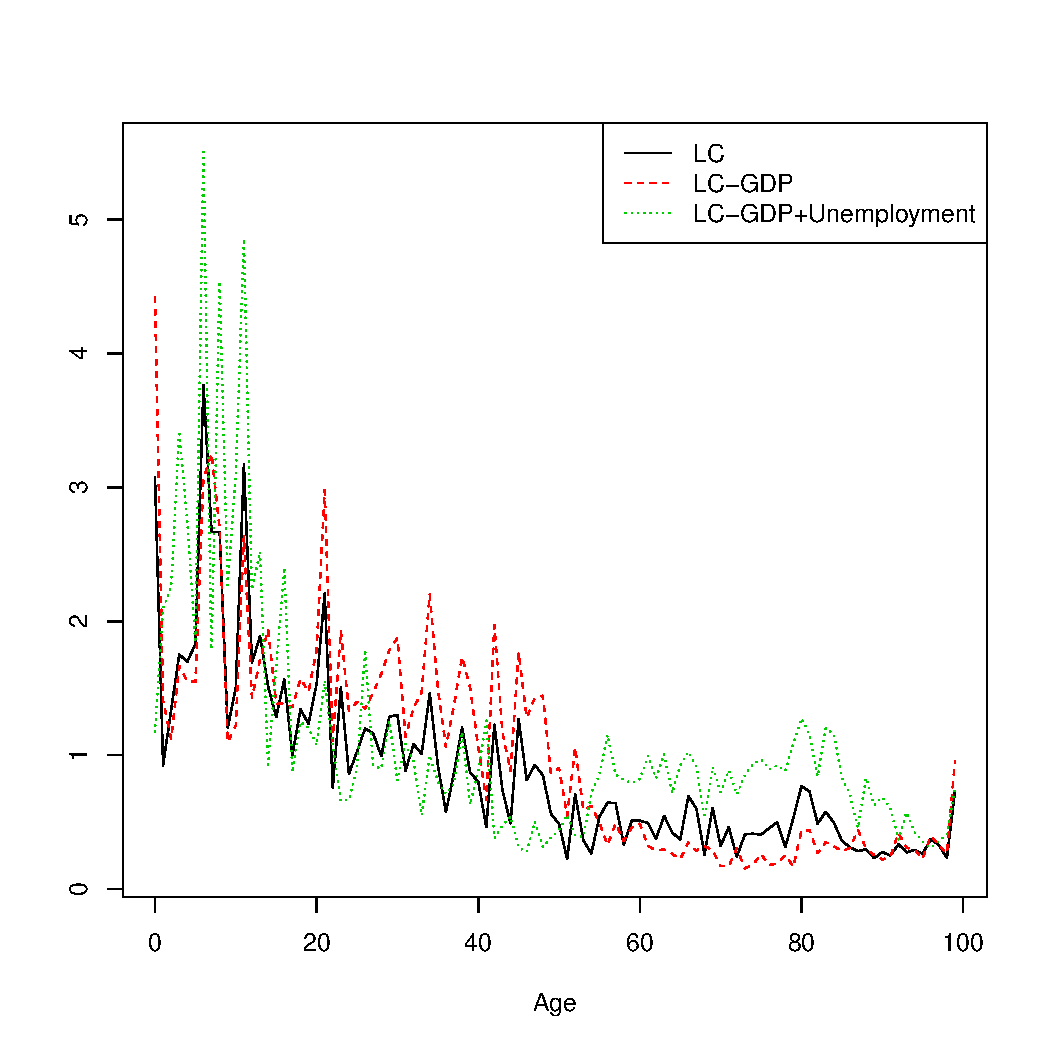
\includegraphics[width=\linewidth]{CAN_abs_pred_error_age_female} 
		\caption{Mean Absolute Error over Time}
	\end{subfigure}
	\begin{subfigure}{0.4\textwidth}
		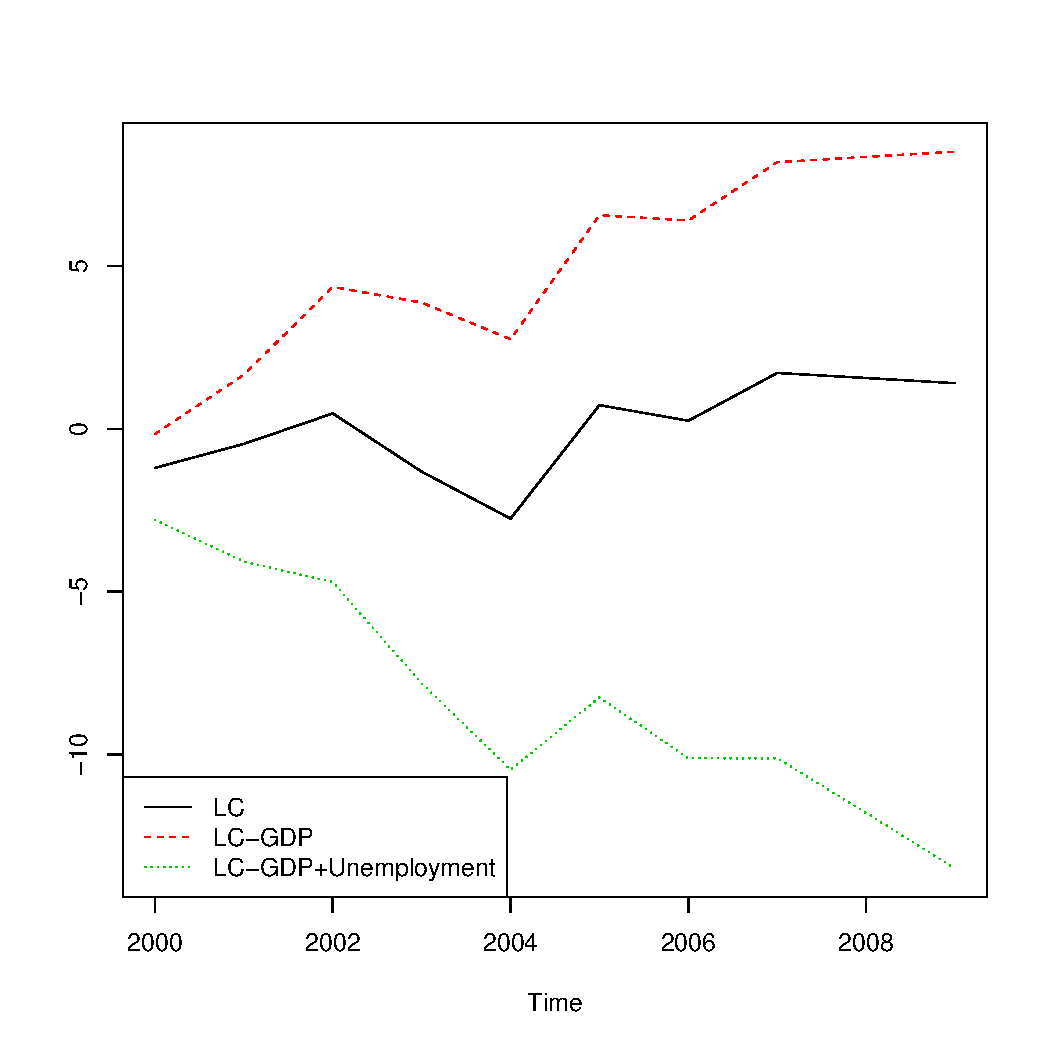
\includegraphics[width=\linewidth]{CAN_pred_error_time_female} 
		\caption{Mean Error over Age}
	\end{subfigure}
	\begin{subfigure}{0.4\textwidth}
		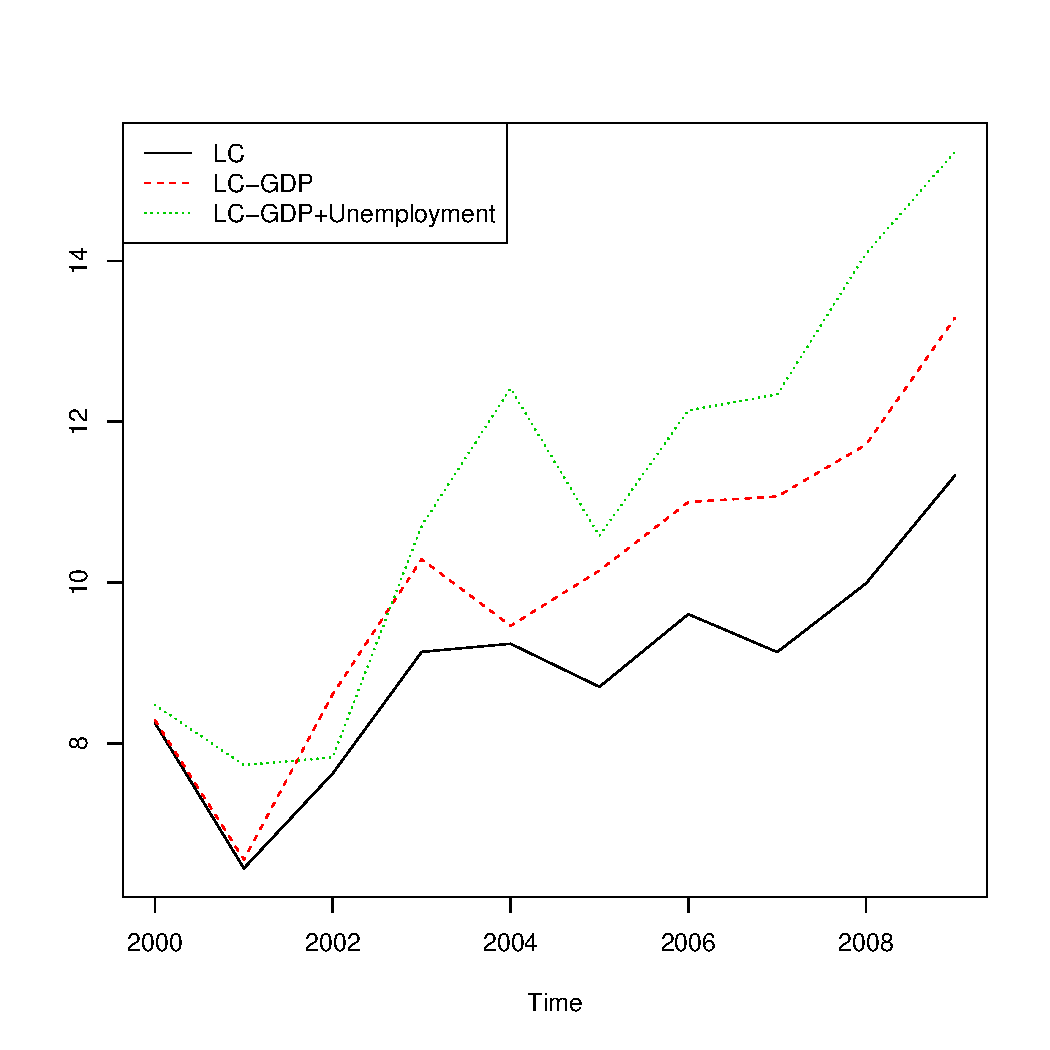
\includegraphics[width=\linewidth]{CAN_abs_pred_error_time_female} 
		\caption{Mean Absolute Error over Age}
	\end{subfigure}
	\caption{Mean error for forecast $\ln(\mu_{xt})$ for Canadian females}
\end{figure}

\end{document}

